%% 
%% Copyright 2007-2020 Elsevier Ltd
%% 
%% This file is part of the 'Elsarticle Bundle'.
%% ---------------------------------------------
%% 
%% It may be distributed under the conditions of the LaTeX Project Public
%% License, either version 1.2 of this license or (at your option) any
%% later version.  The latest version of this license is in
%%    http://www.latex-project.org/lppl.txt
%% and version 1.2 or later is part of all distributions of LaTeX
%% version 1999/12/01 or later.
%% 
%% The list of all files belonging to the 'Elsarticle Bundle' is
%% given in the file `manifest.txt'.
%% 

%% Template article for Elsevier's document class `elsarticle'
%% with numbered style bibliographic references
%% SP 2008/03/01
%%
%% 
%%
%% $Id: elsarticle-template-num.tex 190 2020-11-23 11:12:32Z rishi $
%%
%%
\documentclass[3p, twocolumn, 10pt]{elsarticle}

%% Use the option review to obtain double line spacing
%% \documentclass[authoryear,preprint,review,12pt]{elsarticle}

%% Use the options 1p,twocolumn; 3p; 3p,twocolumn; 5p; or 5p,twocolumn
%% for a journal layout:
%% \documentclass[final,1p,times]{elsarticle}
%% \documentclass[final,1p,times,twocolumn]{elsarticle}
%% \documentclass[final,3p,times]{elsarticle}
%% \documentclass[final,3p,times,twocolumn]{elsarticle}
%% \documentclass[final,5p,times]{elsarticle}
%% \documentclass[final,5p,times,twocolumn]{elsarticle}

%% For including figures, graphicx.sty has been loaded in
%% elsarticle.cls. If you prefer to use the old commands
%% please give \usepackage{epsfig}

%% The amssymb package provides various useful mathematical symbols
\usepackage{bm}
\usepackage{amsmath}
\usepackage{siunitx}
\usepackage{amsfonts}
\usepackage{amssymb}
\usepackage{mathtools}
\usepackage[X2, T1]{fontenc}
\usepackage[utf8]{inputenc}
\usepackage{comment}
%% The amsthm package provides extended theorem environments
%% \usepackage{amsthm}

%% The lineno packages adds line numbers. Start line numbering with
%% \begin{linenumbers}, end it with \end{linenumbers}. Or switch it on
%% for the whole article with \linenumbers.
%% \usepackage{lineno}

\journal{Chemical Engineering Journal}

\begin{document}

\begin{frontmatter}

%% Title, authors and addresses

%% use the tnoteref command within \title for footnotes;
%% use the tnotetext command for theassociated footnote;
%% use the fnref command within \author or \address for footnotes;
%% use the fntext command for theassociated footnote;
%% use the corref command within \author for corresponding author footnotes;
%% use the cortext command for theassociated footnote;
%% use the ead command for the email address,
%% and the form \ead[url] for the home page:
%% \title{Title\tnoteref{label1}}
%% \tnotetext[label1]{}
%% \author{Name\corref{cor1}\fnref{label2}}
%% \ead{email address}
%% \ead[url]{home page}
%% \fntext[label2]{}
%% \cortext[cor1]{}
%% \affiliation{organization={},
%%             addressline={},
%%             city={},
%%             postcode={},
%%             state={},
%%             country={}}
%% \fntext[label3]{}

\title{A novel numerical model of two-phase flow considering multiple bubble sizes in an alkaline water electrolyzer}

%% use optional labels to link authors explicitly to addresses:
%% \author[label1,label2]{}
%% \affiliation[label1]{organization={},
%%             addressline={},
%%             city={},
%%             postcode={},
%%             state={},
%%             country={}}
%%
%% \affiliation[label2]{organization={},
%%             addressline={},
%%             city={},
%%             postcode={},
%%             state={},
%%             country={}}

\author[a]{Ryo Kanemoto}
\author[b]{Takuto Araki}
\author[c,d]{Shigenori Mitsushima}

\affiliation[a]{organization={Graduate School of Engineering Science, Yokohama National University},%Department and Organization
            addressline={79-5}, 
            city={Hodogaya, Yokohama},
            postcode={2408501}, 
            state={Kanagawa},
            country={Japan}}
\affiliation[b]{organization={Faculty of Engineering, Division of Systems Research, Yokohama National University},%Department and Organization
            addressline={79-5}, 
            city={Hodogaya, Yokohama},
            postcode={2408501}, 
            state={Kanagawa},
            country={Japan}}
\affiliation[c]{organization={Institute of Advanced Sciences, Yokohama National University},%Department and Organization
            addressline={79-5}, 
            city={Hodogaya, Yokohama},
            postcode={2408501}, 
            state={Kanagawa},
            country={Japan}}
\affiliation[d]{organization={Green Hydrogen Research Center, Yokohama National University},%Department and Organization
            addressline={79-5}, 
            city={Hodogaya, Yokohama},
            postcode={2408501}, 
            state={Kanagawa},
            country={Japan}}

\begin{abstract}
Precise description of bubble flow behavior is vital to predict the performance of water electrolysis.
This study employed the Euler-Euler model to simulate bubble flow within an alkaline water electrolysis cell. 
The dispersed gas bubble phase was categorized into three bubble size classes with the representative diameters of 30 (small), 90 (medium), and 270 \si{\micro\metre} (large), where velocity and volume fraction fields were calculated for each class.
Simlations were conducted for three current densities and the results highlighted distinct flow field differences among the three size classes.
This behavior can be attributed to the balance between viscous drag and buoyancy force, which scales with the specific surface area of the bubbles.
The simulation results were compared with experimental visualization in terms of the descending height of bubble circulation along the liquid flow.
Additional simulation with only the medium size class was compared to that with three size classes and the necessity of considering multiple size classes was confirmed.
\end{abstract}

%%Graphical abstract
%\begin{graphicalabstract}
%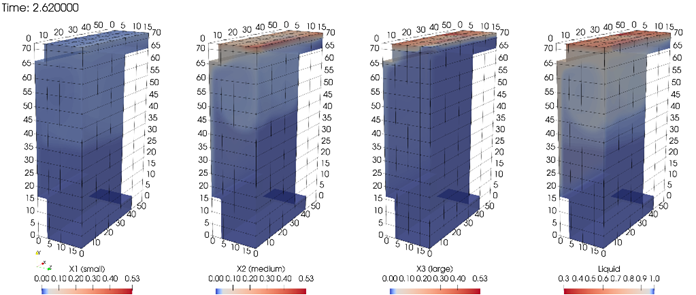
\includegraphics{Untitled 6.png}
%\end{graphicalabstract}

%%Research highlights
\begin{highlights}
\item Simulation of bubble flow in a water electrolyzer for several current densities.
\item Multiple bubble size classes were considered within the framework of Euler-Euler model.
\item Each size class has its own distinct velocity and volume fraction fields.
\item Simulation results were compared to experimental visualizaqtion results.
\item Importance of considering multiple size classes was demonstrated.
\end{highlights}

\begin{keyword}
%% keywords here, in the form: keyword \sep keyword

%% PACS codes here, in the form: \PACS code \sep code

%% MSC codes here, in the form: \MSC code \sep code
%% or \MSC[2008] code \sep code (2000 is the default)
Alkaline water electrolysis, CFD, Two-phase flow, Multiple dispersed phase
\end{keyword}

\end{frontmatter}

%% \linenumbers

%% main text
\section{Introduction}
\label{sec:intro}
Hydrogen, conventionally produced primarily through petroleum refining for various industrial applications, is now drawing attention for its production via water electrolysis due to the growing demand for it as a carrier of renewable energy.
However, the proportion of hydrogen produced through water electrolysis remains relatively very low compared to overall production~\cite{IEA-H2Future}.
This should be addressed by drastically improving the energy efficiency of water electrolysis and lowering the hydrogen costs. 
There are three major types of water electrolysis: proton exchange membrane type, alkaline type, and solid oxide type. 
In order to produce hydrogen with renewable energy, which has a fluctuating and intermittent output, an ideal water electrolysis system must be able to start up in a short time and have a broad load flexibility range~\cite{braunsAlkalineWaterElectrolysis2020}.
In terms of that, proton exchange membrane water electrolysis (PEMWE) seems to be the best option. 
Nevertheless, the major type for large-scale hydrogen production is currently AWE since it offers low investment costs and relies on mature traditional technology. 
While PEMWE uses noble metals like platinum and iridium oxide as its electrocatalysts, AWE uses non-noble metals like nickel and iron, which makes the investment costs of AWE cheaper than those of PEMWE. 
Besides, the lifetime of AWE systems is longer and the annual maintenance costs are lower compared to PEMWE systems~\cite{schmidtFutureCostPerformance2017, buttlerCurrentStatusWater2018}.
However, AWE needs improvement in its dynamic performance. 
% ↓ This might need ref
It is often mentioned that AWE has a long start-up time and a slow dynamic response to the variation of load. 
% ↑ This might need ref
Therefore, the dynamic behavior of AWE must be deeply investigated to design and install much larger scales of hydrogen production systems. 
% ↓ This sentence should be revised
One of the important factors that affect the dynamic response is the presence of bubbles, which can modify the modality of heat and mass transport~\cite{anguloInfluenceBubblesEnergy2020, parkSolutalMarangoniEffect2023}.
% ↑ This sentence should be revised
Especially for the industrial scale of AWE cells, since they are oftentimes long in the direction of gravity, the volume fraction of bubble in the vicinity of the electrodes can vary considerably depending on location, which makes the electrodes experience heterogeneity and can ultimately lead to electrode degradation. 
Therefore, we study the influence of the bubble-liquid flow on the dynamic behavior of the electrochemical performance, for which experimental and computational approaches are available. 
While experimental investigations play a crucial role in understanding the dynamic behavior~\cite{bakkerGasBubbleRemoval2019}
, conducting experiments with industrial scale AWE cells often requires high cost.
Hence, a macroscopic computational approach that models the behavior of an entire cell or stack can be also effective to obtain a comprehensive data about the physical properties of interest.
A computational simulation of an AWE cell is a multiphysics that consists of two main parts: a fluid flow model to describe the mass transport of fluid and an electrochemical model.
Here, in a macroscopic simulation, these two models have to be bridged by another model to consider the interaction between the electrochemical reactions at the electrode surface and the mass transport in the fluid part. 
However, since there is no such model that is well-established yet, our target in this paper is limited to the modelling of the bubble-liquid flow and its evaluation.

Bubble-liquid flow is modeled with two main methods: separated phase models and dispersed phase models~\cite{COMSOLmsmpf1}.
The separated phase models, which include interface capturing method and interface tracking method, are useful when simulating the detailed surface motion of bubbles.
However, for an industrial scale AWE cell, the separated phase models require huge computational cost, thus making the dispersed phase models more desirable.
Among the several dispersed phase models, the Euler-Euler model is suitable to deal with a large number of particles and momentum exchanges between bubbles and liquid.

For the particle size of the dispersed phase, monodisperse size distribution is selected in some cases~\cite{jupudiModelingBubbleFlow2009, dreoniAccuracyAssessmentEulerian2022, bideauEulerianTwoFluidModel2020}.
However, since the size variation of electrochemically generated bubbles is so large~\cite{ikedaMicroscopicHighspeedVideo2022,wedinExperimentsModellingElectrochemically2003,boissonneauBubbleInducedFree2000}
that monodisperse models~\cite{bideauEulerianTwoFluidModel2020, zarghamiCFDModelingMultiphase2020, alexiadisLiquidgasFlowPatterns2011}
are inadequate to deal with the difference in the behavior of different size bubbles, polydisperse models are more appropriate for the bubble-liquid flow inside a water electrolyzer.
As a part of polydisperse models, population balance model (PBM) has been studied by many researchers and various types of PBMs have been developed~\cite{liQuadraturebasedMomentMethods2019}.

The basic concepts behind PBM is to consider the conservation of number density function by solving a population balance equation.
Here, number density function represents the number distribution of dispersed particle size (usually volume or diameter).
By extracting Sauter diameters from the number density function and use them in the Euler-Euler model CFD simulation, the detailed flow fields for different particle sizes can be estimated.

The existing studies of CFD simulations coupled with PBM have provided valid and accurate results in polydisperse systems.
However, most of those studies deal only with bubble columns as their targets to apply PBM.
While bubble column reactors sometimes even have a circulation flow by having components that induce a downward flow, to our best knowledge, no studies have applied PBM to bubble columns with circulation flow~\cite{chenCFDModelingBubble2004,bholeCFDSimulationBubble2008,sanyalComparisonPopulationBalance2004,liuCultivationAerobicGranules2007}.
In general, water electrolyzers have a circulation flow inside them, and since electrochemically generated bubbles have a wide range of size distribution, the velocity fields for each bubble size are often different from one another.
Since PBM has only a single momentum equation for the entire dispersed phase, it is not easy to accurately simulate flow systems where there are significant variations in velocity fields depending on the different sizes of the dispersed phase.

Therefore, in this paper, we introduce a polydisperse model that holds multiple size classes, each of which has its own momentum equation so that the different velocity fields are simulated for different size classes.
This feature allows for simulating flow fields with significant variations not only in the magnitude but also even in the direction of velocity fields for each particle size class.
Using this model, we focused on simulating the bubble-liquid flow field in an alkaline water electrolysis cell.

\section{Physical Setup}
Fig.\ref{fig:exp.cell} shows anode side of the alkaline water electrolysis cell used for validation of the presented 
CFD model. Note that we focus on the fluid flow field, which we do not consider; This cell is zero-gap mono-polar 
type and only its anode side is considered in the simulation, since this study's target is the fluid flow field. 
The potassium hydroxide solution (KOH) was pumped from the inlet at the bottom of the acrylic case and flows out 
from the outlet in the middle. Since this cell was primarily designed to investigate local electrochemical behavior, 
the nickel expanded metal electrode is divided into two parts: the main electrode and a smaller electrode, although 
the latter was not used in this study. As electric current is applied, oxygen bubbles are generated from the main 
electrode. The measurements for validation were performed at the following three current densities: 
$j=0.3$, $0.6$, $1.0$ $[\mathrm{A/cm^2}]$.


\begin{figure}[h]
  \centering
  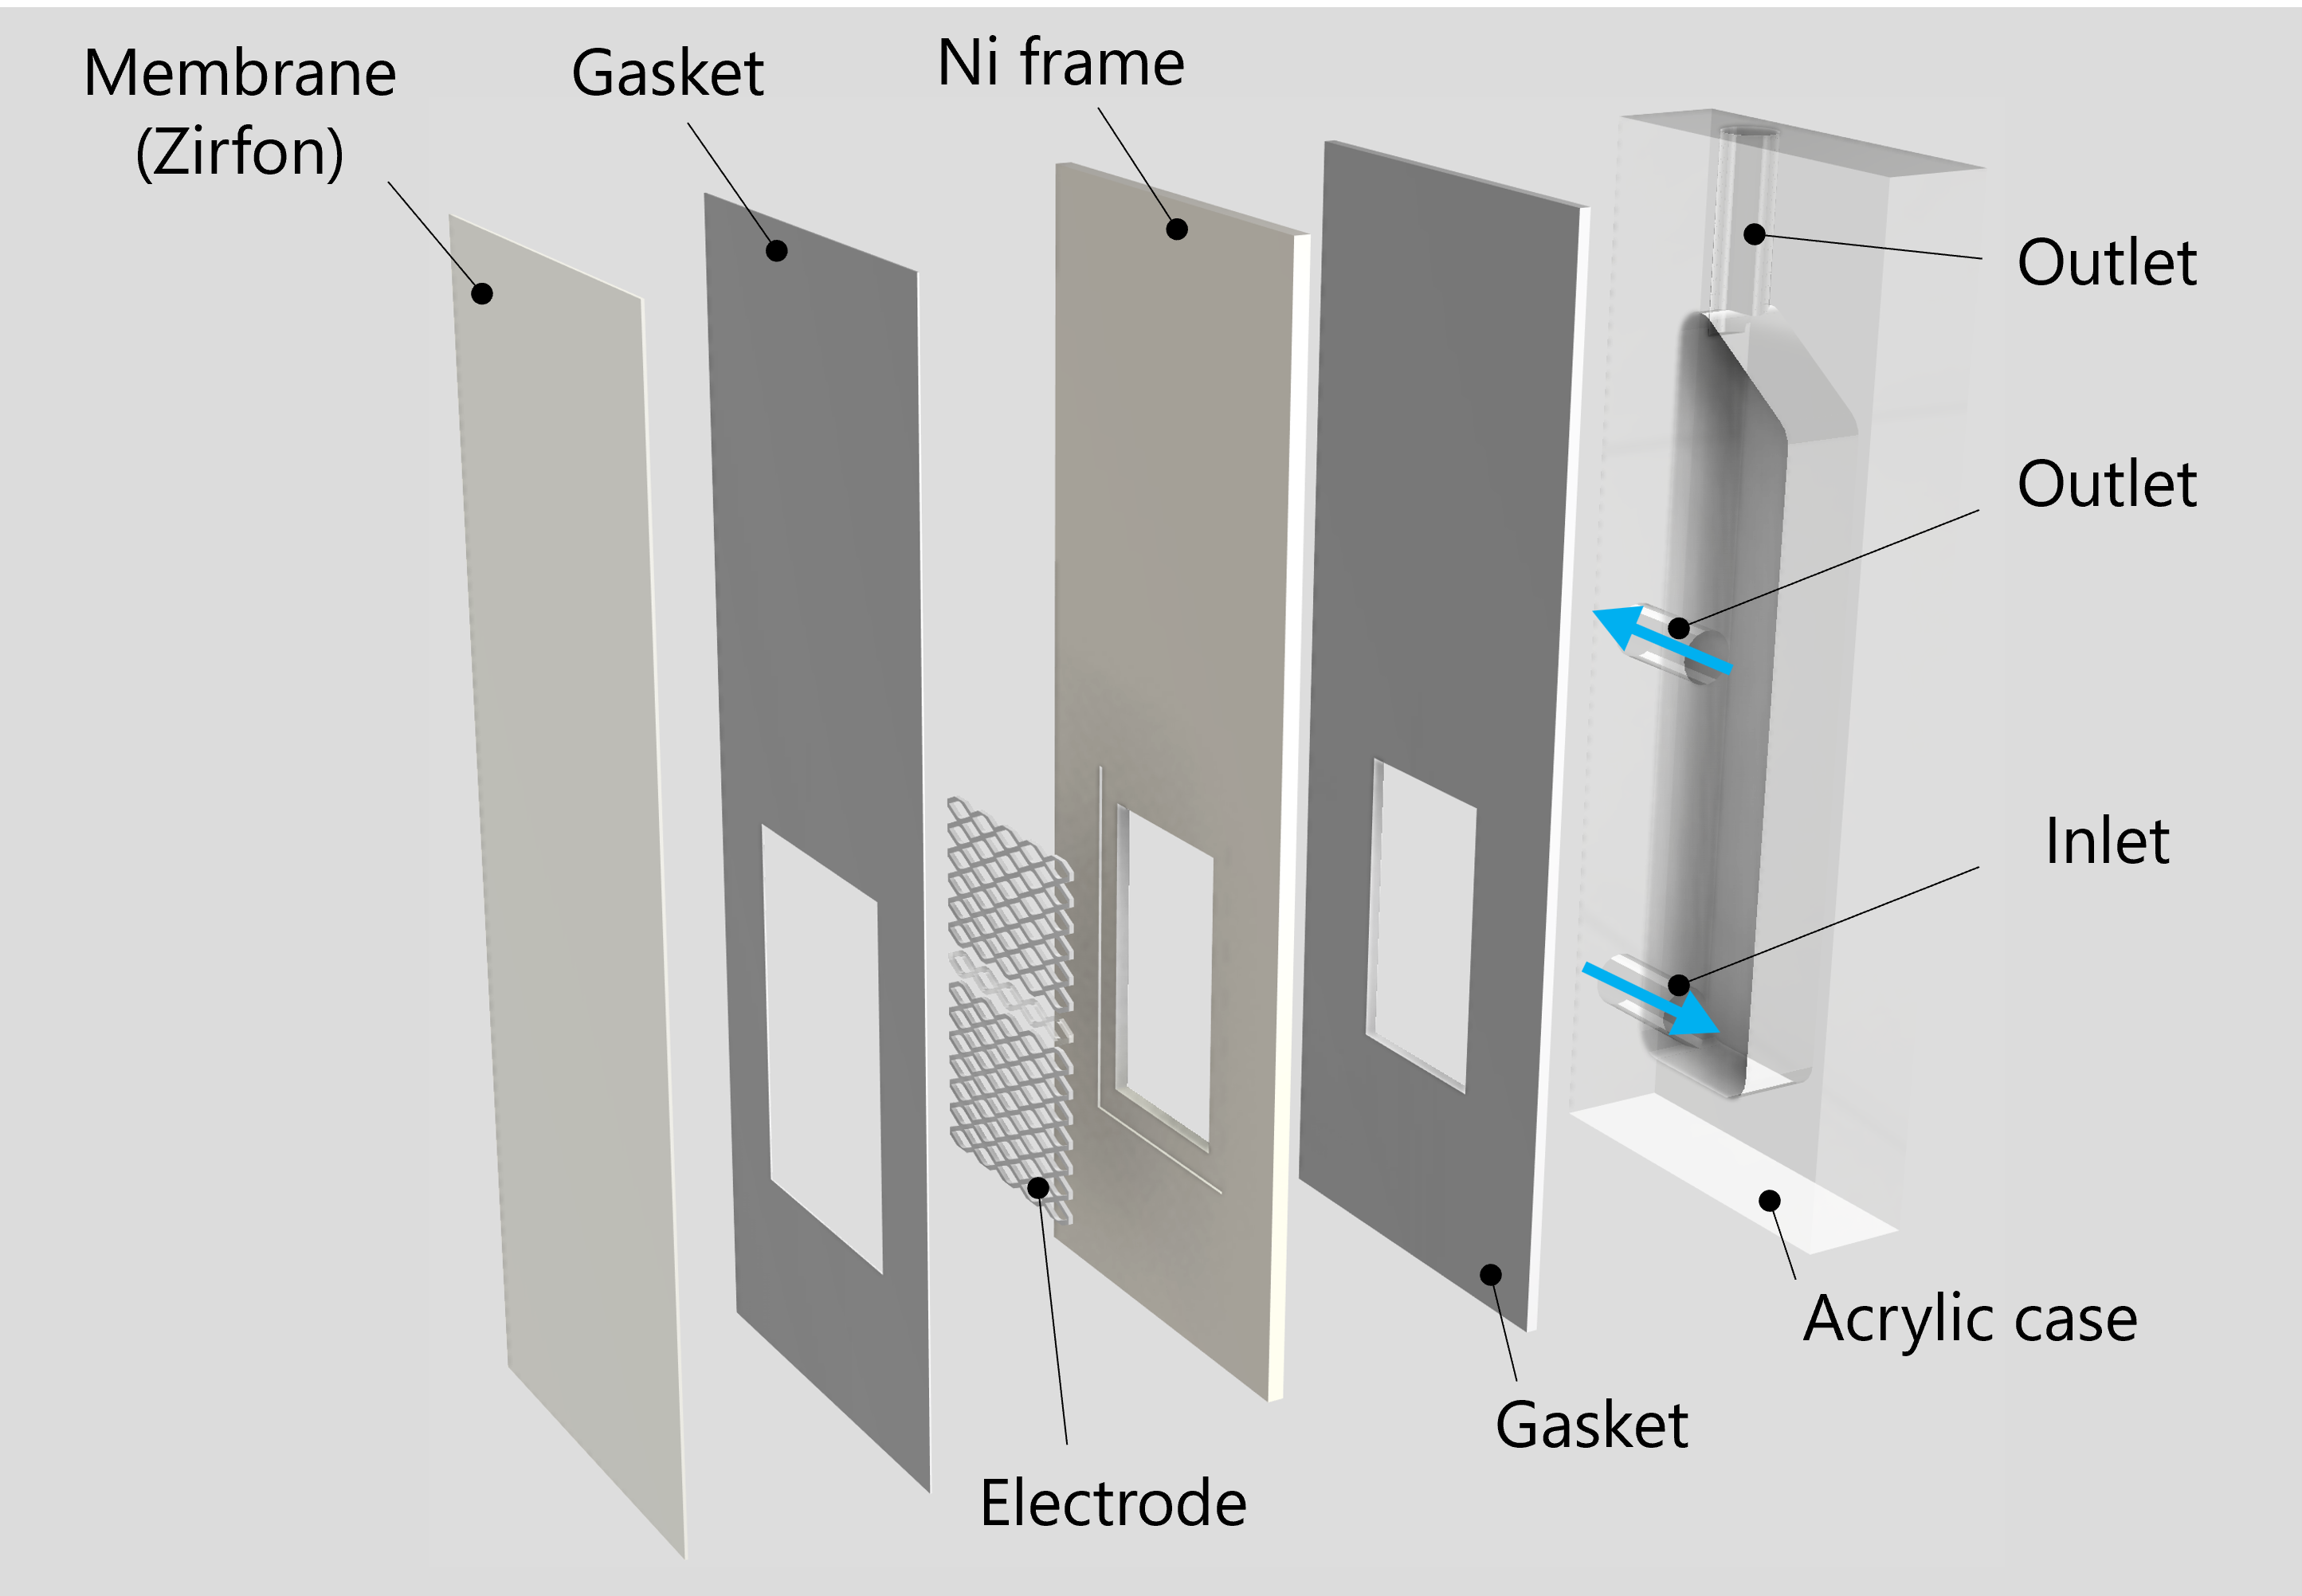
\includegraphics[width=1\linewidth]{Untitled.png}
  \caption{Configuration of the experimental AWE anodic half-cell, with electrolyte flow indicated by the blue arrows indicate. The smaller electrode is rendered as transparent since it was not in use. Some components are omitted for simplicity.}
  \label{fig:exp.cell}
\end{figure}

\section{Governing equations}
The simulation of bubble-liquid flow in an alkaline water electrolyzer in this work was performed using reactingMultiphaseEulerFoam, a multiphase flow solver in OpenFOAMv2006 based on the Eulerian model~\cite{OpenFOAMrmef}.
This solver can deal with multiple different fluid components to simulate a multiphase flow involving chemical reactions, and the velocity fields can be calculated for each different component.
Although this study does not explicitly deal with chemical reactions, this feature can be exploited to calculate the velocity fields for the bubbles of each different size class by considering each bubble size group as a separate component.
Thus, in the bubble-liquid flow simulation, when we introduce $N$ classes of bubble size, all we consider are $N$ gas phases and one liquid phase, i.e., a total of $N+1$ phases.
Each of the phases has its own phase fraction field, and they satisfy the following equation:

\begin{align}\label{eq:alphasum}
  \sum_{i}^N\alpha_{i} + \alpha_{l}=1,
\end{align}
where $\alpha$ is the phase volume fraction, and the subscripts $i$ and $l$ represent the bubble size class and the liquid phase, respectively.
The continuity and momentum equations are written as:
\begin{align}\label{eq:continuity_i}
  \dfrac{\partial}{\partial t}
  \left(
  \alpha_{i}\rho_{i}
  \right)+
  \nabla
  \left(
  \alpha_{i}\rho_{i}\bm{u}_{i}
  \right)=
  \dot{m}_{i},
\end{align}
\begin{align}
    \dfrac{\partial}{\partial t}
    \left(
    \alpha_{i}
    \rho_{i}\bm{u}_{i}
    \right)&+
    \nabla\cdot
    \left(
    \alpha_{i}\rho_{ i}\bm{u}_{i}\bm{u}_{i}
    \right)\notag \\
    &=
    -\alpha_{i}\nabla p +
    \nabla\cdot
    \left(
    \alpha_{i}\tau_{i}
    \right)
    +
    \alpha_{i}\rho_{i}g
    +M_{il}
\end{align}
for the bubble size class $i$, and
\begin{align}
  \dfrac{\partial}{\partial t}
  \left(
  \alpha_{l}\rho_{l}
  \right)+
  \nabla
  \left(
  \alpha_{l}\rho_{l}\bm{u}_{l}
  \right)=0,
\end{align}
\begin{align}
  \dfrac{\partial}{\partial t}
  \left(
  \alpha_{l}\rho_{l}\bm{u}_{l}
  \right)&+
  \nabla\cdot
  \left(
  \alpha_{l}\rho_{ l}\bm{u}_{l}\bm{u}_{l}
  \right)\notag \\
  &=
  -\alpha_{l}\nabla p +
  \nabla\cdot
  \left(
  \alpha_{l}\tau_{l}
  \right)
  +
  \alpha_{l}\rho_{l}g
  -M_{il}
\end{align}
for the liquid phase $l$.
Here, the momentum equation for the liquid phase is Reynolds averaged and the Reynolds stress is modeled by the standard $k$-$\varepsilon$ model.
In these equations, $\rho$ is phase density, $\bm{u}$ is phase velocity vector, $g$ is the gravitational acceleration, and $\dot{m}_i$ is a volumetric mass source term that is only active in the computational cells facing the electrode boundary, which is explained in Section \ref{sec:boundaryConditions}. 
Also, $\tau$ is the stress tensor, which is expressed as
\begin{align}
  \tau_{} = \mu_{}^\mathrm{}
  \left\{
  2\bm{D}_{}-
  \dfrac{2}{3}
  \mathrm{tr}
  \left(\bm{D}_{}\right)\bm{I}
  \right\},
\end{align}
where $D$ is the strain rate tensor described as
\begin{align}
  \bm{D}_{} =
  \dfrac{1}{2}
  \left\{
  \nabla\bm{u}_{}+
  \left(
  \nabla\bm{u}_{}
  \right)^\mathrm{T}
  \right\}.
\end{align}
The viscosity $\mu$ is defined as $\mu_{i} = \mu_{g}^{\mathrm{mol}}$ for the gas 
phases and $\mu_{l}=\mu_{l}^{\mathrm{mol}}+\mu_{l}^{\mathrm{turb}}$ for the liquid 
phase, where $\mu^{\mathrm{mol}}$ is the molecular dynamic viscosity of the phase, 
and $\mu^{\mathrm{turb}}$ is the turbulent viscosity (or eddy viscosity). Since we 
used the standard $k$-$\varepsilon$ model, the turbulent viscosity is estimated as
\begin{align}
  \mu_{l}^{\mathrm{turb}} = C_{\mu}\dfrac{\rho_{l}k^2}{\varepsilon},
\end{align}
where $k$ is turbulent kinetic energy and $\varepsilon$ is turbulent energy 
dissipation rate. 
\begin{comment}
  The transport equation is expressed as
\begin{align}
  \dfrac{\partial \alpha_{l}\rho_{l}k}{\partial t}
  & + 
  \nabla\cdot\left(
  \alpha_{l}\rho_{l}k \bm{u_{l}}
  \right)\\
  & =
  \nabla\cdot
  \left\{
  \left(
  \dfrac{\nu_{l}^{\mathrm{turb}}}{\sigma_{k}}+\nu_{l}^{\mathrm{
  mol}}
  \right)
  \nabla\left(
  \alpha_{l}\rho_{l}k
  \right)
  \right\}
  +
  \alpha_{l}G-\alpha_{l}\rho_{l}\varepsilon,
\end{align}
for the turbulent kinetic energy and
\begin{align}
  \dfrac{\partial \alpha_{l}\rho_{l}\varepsilon}{\partial t}
  & + 
  \nabla\cdot\left(
  \alpha_{l}\rho_{l}\varepsilon \bm{u_{l}}
  \right)\\
  & =
  \nabla\cdot
  \left\{
  \left(
  \dfrac{\nu_{l}^{\mathrm{turb}}}{\sigma_{\varepsilon}}+\nu_{l}^{\mathrm{
  mol}}
  \right)
  \nabla\left(
  \alpha_{l}\rho_{l}\varepsilon
  \right)
  \right\}
  +
  \alpha_{l}\dfrac{\varepsilon}{k}
  \left(
  C_{1\varepsilon}G
  -
  C_{2\varepsilon}\rho_{l}\varepsilon
  \right)
\end{align}
for the turbulent energy dissipation rate, where $\nu_{l}=\mu_{l}/\rho_{l}$ is the kinematic viscosity and $G$ is the production of turbulence kinetic energy. 
The constant coefficients $C_{\mu}$, $\sigma_{k}$, $\sigma_{\varepsilon}$, $C_{1\varepsilon}$, $C_{2\varepsilon}$ are $0.09$, $1.0$, $1.3$, $1.44$, $1.92$, respectively.
\end{comment}

We considered the momentum transfer between the bubble size class $i$ and the liquid phase as $M_{il}$ in each momentum transport equation, which is the summation of drag $\left(F_{\mathrm{D}}\right)$, virtual mass $\left(F_{\mathrm{VM}}\right)$, lift $\left(F_{\mathrm{L}}\right)$, wall lubrication $\left(F_{\mathrm{WL}}\right)$, turbulent dispersion $\left(F_{\mathrm{TD}}\right)$ forces:
\begin{align}
  M_{il} = F_{\mathrm{D}}+
  F_{\mathrm{VM}}+
  F_{\mathrm{L}}+
  F_{\mathrm{WL}}+
  F_{\mathrm{TD}}
\end{align}

The drag force $F_{\mathrm{D}}$ results from the viscosity of the continuous phase when the dispersed phase has a slip-velocity against the continuous phase and it acts in the opposite direction of the slip-velocity.
\begin{align}
  F_{\mathrm{D}} = - \dfrac{3}{4}\dfrac{C_{\mathrm{D}}}{d_{i}}
  \alpha_{i}\rho_{l}
  \left|\bm{u}_{i} - \bm{u}_{l}\right|
  \left(\bm{u}_{i} - \bm{u}_{l}\right),
\end{align}
where $\bm{u}_{i} - \bm{u}_{l}$ represents the slip-velocity of the bubble class $i$ against the liquid phase $l$, $d_{i}$ is the diameter of the bubble class $i$, and $C_{\mathrm{D}}$ is the drag coefficient which is determined by Schiller and Naumann model~\cite{schillerDrag1933}:
\begin{align}
  C_{\mathrm{D}} =
  \begin{dcases}
  \dfrac{24}{Re_\mathrm{b}}\left(1+0.15Re_\mathrm{b}^{0.687}\right) & \quad \left(Re_\mathrm{b}\leq 1000\right)\\
  0.44                                        & \quad \left(Re_\mathrm{b}> 1000\right)\\
  \end{dcases}
\end{align}
where $Re_\mathrm{b}$ is the Reynolds number of the bubble $Re_\mathrm{b}=\rho_{l}\left|\bm{u}_{i}-\bm{u}_{l}\right|d_{i}/\mu_{l}$. 
The Schiller and Naumann model is applied to spherical particles.
This study deals with the microscale bubbles, whose Eötvös number is sufficiently small that the bubbles can be considered spherical.

The virtual mass (or added mass) force $F_{\mathrm{VM}}$ is generated when the dispersed particles are accelerated relative to the continuous phase~\cite{drewAnalysisVirtualMass1979}.
The relative acceleration of a particle results in carrying some volume of the surrounding fluid along with it, which in turn increases the effective inertia of the particle.
The virtual mass force is expressed as: 
\begin{align}
  F_{\mathrm{VM}} = C_{\mathrm{VM}}\alpha_{i}\rho_{l}
  \left(
  \dfrac{\mathrm{D}\bm{u}_{i}}{\mathrm{D}t}
  -
  \dfrac{\mathrm{D}\bm{u}_{l}}{\mathrm{D}t}
  \right),
\end{align}
where $C_{\mathrm{VM}}$ is the virtual mass coefficient, which is known to be $0.5$ for a spherical particle.

The lift force $F_{\mathrm{L}}$ accounts for the transversal motion of the dispersed particles due to the velocity gradients in the continuous phase~\cite{drewVirtualMassLift1987}, which is expressed as:
\begin{align}
  F_{\mathrm{L}} = C_{\mathrm{L}}\alpha_{i}\rho_{l}
  \left(\bm{u}_{i}-\bm{u}_{l}\right)
  \times
  \left(\nabla\times\bm{u}_{l}\right),
\end{align}
where $C_{\mathrm{L}}$ is the lift coefficient, which is set to $0.5$.

The wall lubrication force $F_{\mathrm{WL}}$ was incorporated to mitigate the overestimation of the gas volume fraction near the wall, where the velocity boundary layer exists around the bubbles.
Without this force, the velocity gradients near the wall cause a dominance of the lift force, which makes the bubbles get overly pushed towards the wall.
We adopted the wall lubrication model derived by Antal et al.~\cite{antalAnalysisPhaseDistribution1991}, which is expressed as:
\begin{align}
  F_{\mathrm{WL}} = 
  \dfrac{C_{\mathrm{WL}}}{d_{i}}
  \alpha_{i}\rho_{l}
  \left|
  \left(
  \bm{u}_{i}-\bm{u}_{l}
  \right)_{||}
  \right|^{2}\bm{n}_{\mathrm{W}},
\end{align}
where $\left(\bm{u}_{i}-\bm{u}_{l}\right)_{||}$ is the bubble relative velocity component tangential to the wall, $\bm{n}_{\mathrm{W}}$ is the normal vector of the wall with the inward direction, and $C_{\mathrm{WL}}$ is the wall lubrication coefficient:
\begin{align}
  C_{\mathrm{WL}} = \mathrm{max}
  \left(0, C_{\mathrm{w1}}+C_{\mathrm{w2}}\dfrac{d_{i}}{2y_{\mathrm{w}}}\right),
\end{align}
where $y_{\mathrm{W}}$ is the distance to the nearest wall, and $C_{\mathrm{w1}}$ and $C_{\mathrm{w2}}$ are the constant coefficients with adopted values of $-0.1$ and $0.15$, respectively.

The turbulent dispersion force $F_{\mathrm{TD}}$ was employed to include the influence of the turbulent random fluctuations on the redistribution of bubbles in the transversal direction~\cite{lubchenkoMoreFundamentalWall2018}.
We used the model derived by Burns~\cite{burnsTheFavreAveragedDrag2004}, which is expressed as:
\begin{align}
  F_{\mathrm{TD}}=-\dfrac{3}{4}
  \dfrac{C_{\mathrm{D}}}{d_{i}}
  \alpha_{i}
  \left|
  \bm{u}_{i}-\bm{u}_{l}
  \right|
  \dfrac{\mu_{l}^{\mathrm{turb}}}{Sc_{\mathrm{TD}}}
  \left(
  \dfrac{1}{\alpha_{i}}
  +\dfrac{1}{1-\alpha_{i}}
  \right)
  \nabla\alpha_{i},
\end{align}
where $Sc_{\mathrm{TD}}$ is the Schmidt number of turbulent dispersion, which is set to $1.0$. 

Note that we assumed bubbles do not to break up or coalesce in the entire simulation domain.
Firstly, the bubbles of interest in this paper are on the microscale and threfore not prone to breaking up easily.
Secondly, coalescence does not occur frequently in the bulk, where the spacing between any bubble pairs is often ample~\cite{hreizElectrogeneratedBubblesInduced2015,leeMicrofabricatedElectrolyticMicrobubblers2005}.
However, coalescence admittedly occurs in the vicinity of electrode or at the areas where bubbles accumulate, such as free liquid surface or ceilings.
As for the vicinity of the electrode, the bubble diameters to be inputted to the simulation are those of bubbles that have already coalesced with other bubbles and detached from the electrode surface (see Section \ref{sec:bubbleSizeClasses}), so a particular coalescence model does not have to be used.
Regarding the areas where bubbles accumulate, since they are densely populated with a high frequency of coalescence events, it is better to have some coalescence model.
Nevertheless, modelling bubble coalescence is not within the scope of this paper, so any coalescence is not considered.

\section{Boundary conditions}\label{sec:boundaryConditions}
The simulation geometry is shown in Fig. \ref{fig:sim.geometry}.
The uniform velocity boundary condition is applied to very phase at the inlet boundary, which is $\bm{u}_{i}=(-0.032,\,0,\,0)\,\mathrm{[m/s]}$.
At the outlet boundary, a constant pressure condition is applied.
All the other boundaries including the top face of the geometry are set as no-slip wall boundaries.
For every phase volume fraction field, zero-gradient condition is applied to all the boundaries.

The volumetric mass source for the bubble class $i$ in Eq. \ref{eq:continuity_i} is defined as:
\begin{align}
  \dot{m}_{i}=
  c_{i}\dfrac{jM}{C_{\mathrm{reac}}F},
\end{align}
where $j$ is the current density, $M$ is the molar mass of the product chemical specie, $C_{\mathrm{reac}}$ is the number of electrons that is required to produce one molecule of the product chemical specie, and $F$ is Faraday's constant.
The fractional part composed of these quantities gives the total mass of the chemical species produced by the electrochemical reaction.
To allocate this total mass to each bubble size class $i$, allocation coefficient $c_{i}$ is multiplied.
Accordingly, the sum of $c_{i}$ must be equal to 1.
Note that the mass of water vapor inside bubbles is negligible since the saturation vapor pressure is very low at the temperature of interest, which is $25\ ^\circ\mathrm{C}$. In addition, we considered the bubbles' initial velocity at the electrode as zero.

Here, the outlet boundary is extended sufficiently further from the electrode because the pressure boundary at the outlet leads to reverse flow, which causes a violation of Eq. \ref{eq:alphasum}.
In Fig. \ref{fig:sim.geometry}, however, the outlet is only displayed up to the necessary length.
\begin{figure}[h]
  \centering
  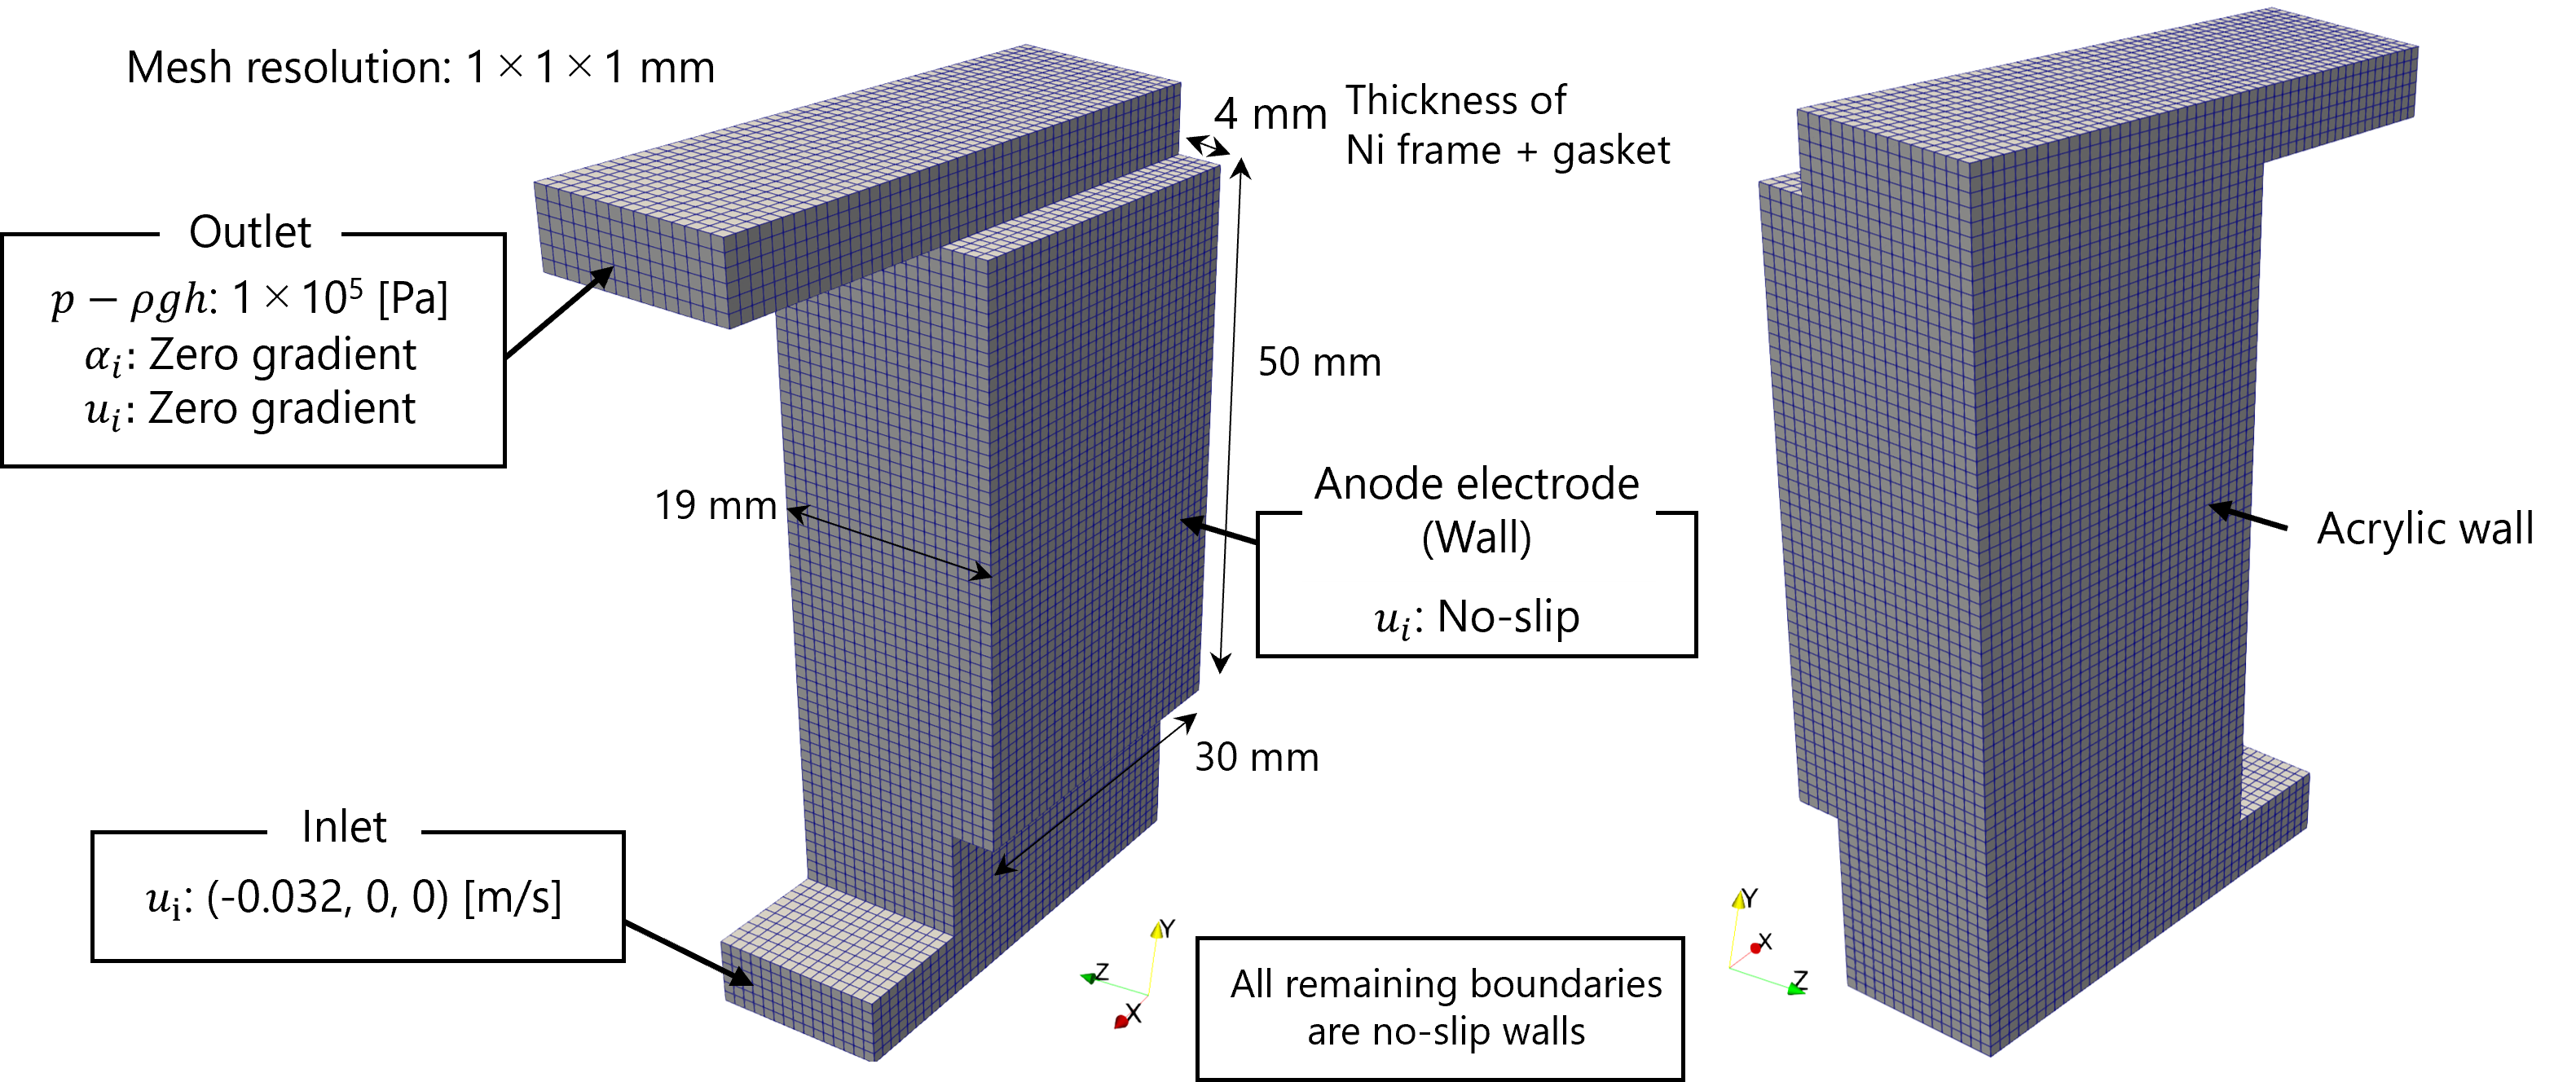
\includegraphics[width=1\linewidth]{Picture3.png}
  \caption{Simulation geometry of the anodic half-cell, where oxygen is produced, and the boundary conditions for main fields.}
  \label{fig:sim.geometry}
\end{figure}

\section{Bubble size classes}\label{sec:bubbleSizeClasses}
In this study, three size classes $\mathrm{X1}$, $\mathrm{X2}$, and $\mathrm{X3}$ were considered.
The representative bubble diameter $d_{i}$ for bubble size class $i=\mathrm{X1}$, $\mathrm{X2}$, or $\mathrm{X3}$ and its allocation coefficient $c_{i}$ were determined based on an experimental visualization.
Fig. \ref{fig:electrode_vid} shows a random frame from the visualized video.
The video was recorded at $6000$ fps, $1024\times 1024$ pixels, and shows the bottom $4\ \mathrm{mm}$ square of the electrode, giving a resolution of $3.9\,\si{\micro\metre}/\mathrm{pixel}$.
In the video, a control surface with its normal vector parallel to the direction of gravity is set.
The diameters of all bubbles passing through the control surface within a randomly selected 0.02 seconds were recorded.
Three sets of this procedure (i.e., $0.06$ seconds in total) were performed at each current density.
\begin{figure}[h]
  \centering
  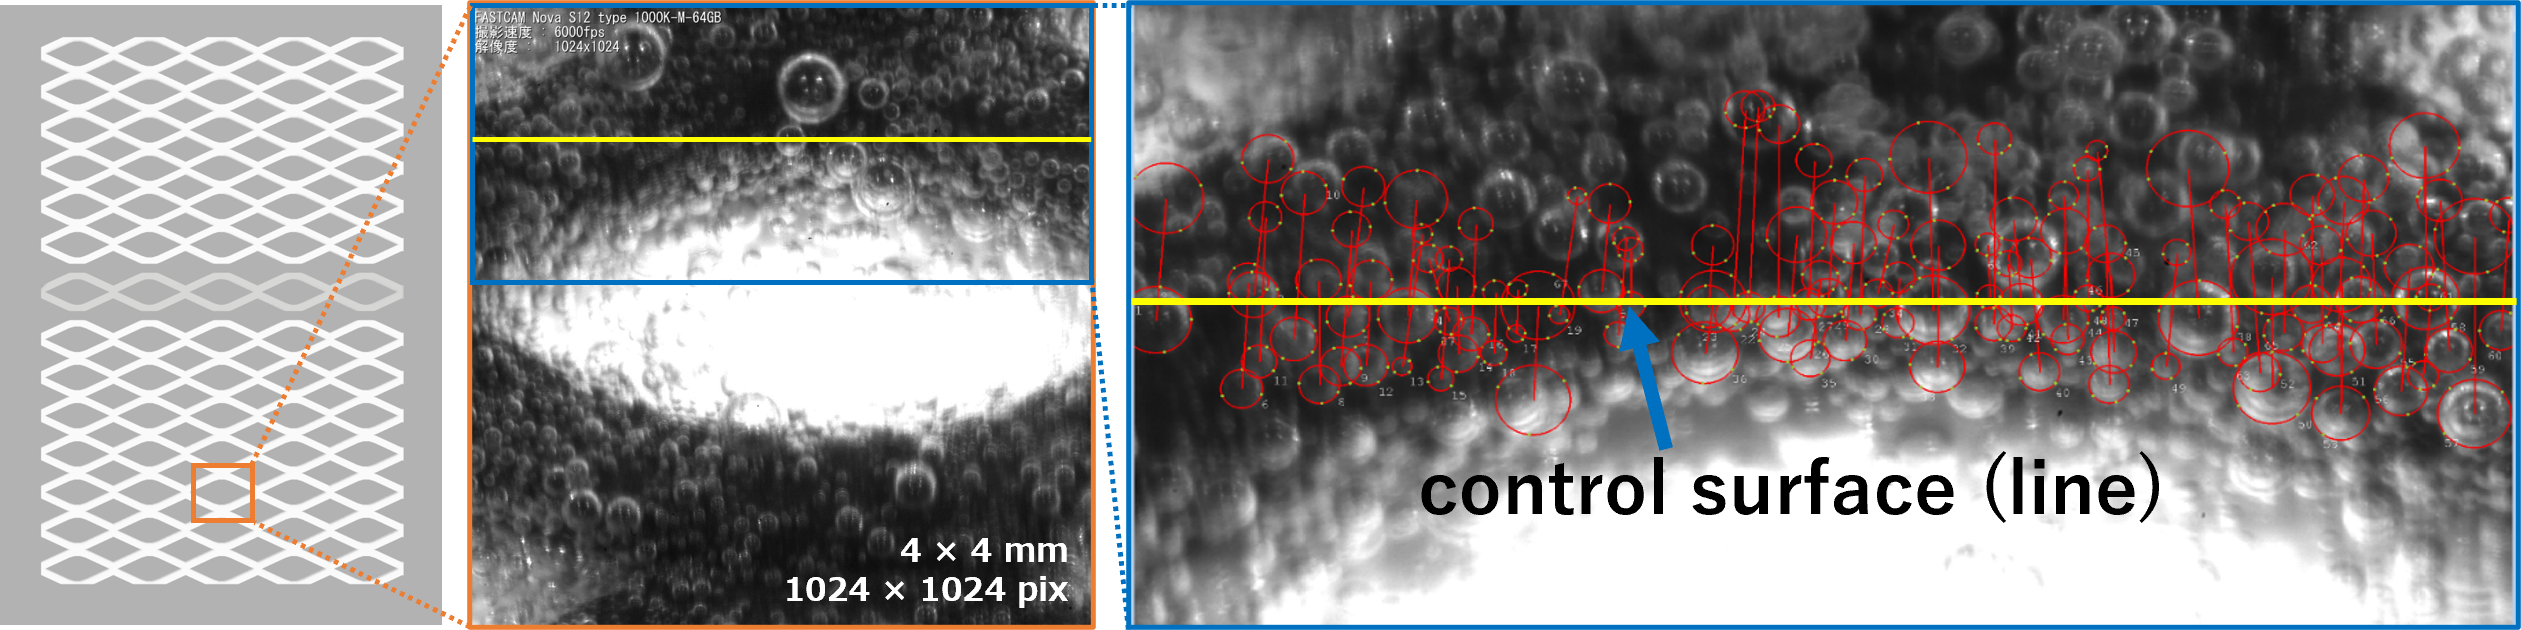
\includegraphics[width=1\linewidth]{Picture1.png}
  \caption{Measurement of bubble diameter from the experimental visualization. }
  \label{fig:electrode_vid}
\end{figure}

To obtain the mass of each bubble, equation of state was considered:
\begin{align}\label{eq:eqofstate}
  P_{\mathrm{in}}\dfrac{4}{3}\pi
  \left(
  \dfrac{d}{2}
  \right)^3 =
  \dfrac{m}{M}RT,
\end{align}
where $P_{\mathrm{in}}$ is the pressure inside the bubble, $d$ is the bubble diameter measured in the experimental videos, $m$ is the bubble mass, $M$ is the molar mass of oxygen, $R$ is the gas constant, $T$ is the temperature of gas, which is $25\ ^\circ\mathrm{C}$.
Besides, $P_{\mathrm{in}}$ is calculated using the following Young-Laplace equation:
\begin{align}\label{eq:yl}
  P_{\mathrm{in}}=P_{\mathrm{out}}
  +\dfrac{2\gamma}{d/2},
\end{align}
where $P_{\mathrm{out}}$ is the pressure outside the bubble, $\gamma$ is the surface tension of alkaline liquid, which is considered to be almost equal to that of water.
Eq. \ref{eq:eqofstate} and \ref{eq:yl} yield the mass $m$ of the bubble with diameter $d$.
Thus, the diameter distribution (Fig. \ref{fig:histogram}a) is converted to the mass distribution (Fig. \ref{fig:histogram}b).
Here, to divide the mass distribution into three size classes, the size class boundaries $\mathrm{X1}\textit{-}\mathrm{X2}$ and $\mathrm{X2}\textit{-}\mathrm{X3}$ are set at $60\,\si{\micro\metre}$ and $180\,\si{\micro\metre}$, respectively.
The representative diameters of $\mathrm{X1}$, $\mathrm{X2}$, and $\mathrm{X3}$ are set to $30$, $90$, and $270\,\si{\micro\metre}$, respectively.
These parameters for the class boundaries and the representative diameters were selected to make the discussion simple.
Note that selecting the average diameter of a size class, which can be obtained by calculating the average mass of the size class and substituting it into Eq. \ref{eq:eqofstate}, as its representative diameter was also an option.
However, we chose to fix the representative diameters over all the current density conditions in order to make the discussion simple.
Hence, for a given size class $i$, the representative diameter $d_{i}$ remains constant regardless of current density, while the mass allocation coefficient $c_{i}$, calculated as the ratio of the total mass of the size class $i$ to the total mass of all the size classes, varies with the current density.
The calculated $c_{i}$ is summarized in Fig. \ref{fig:ci}.
\begin{figure}[h]
  \centering
  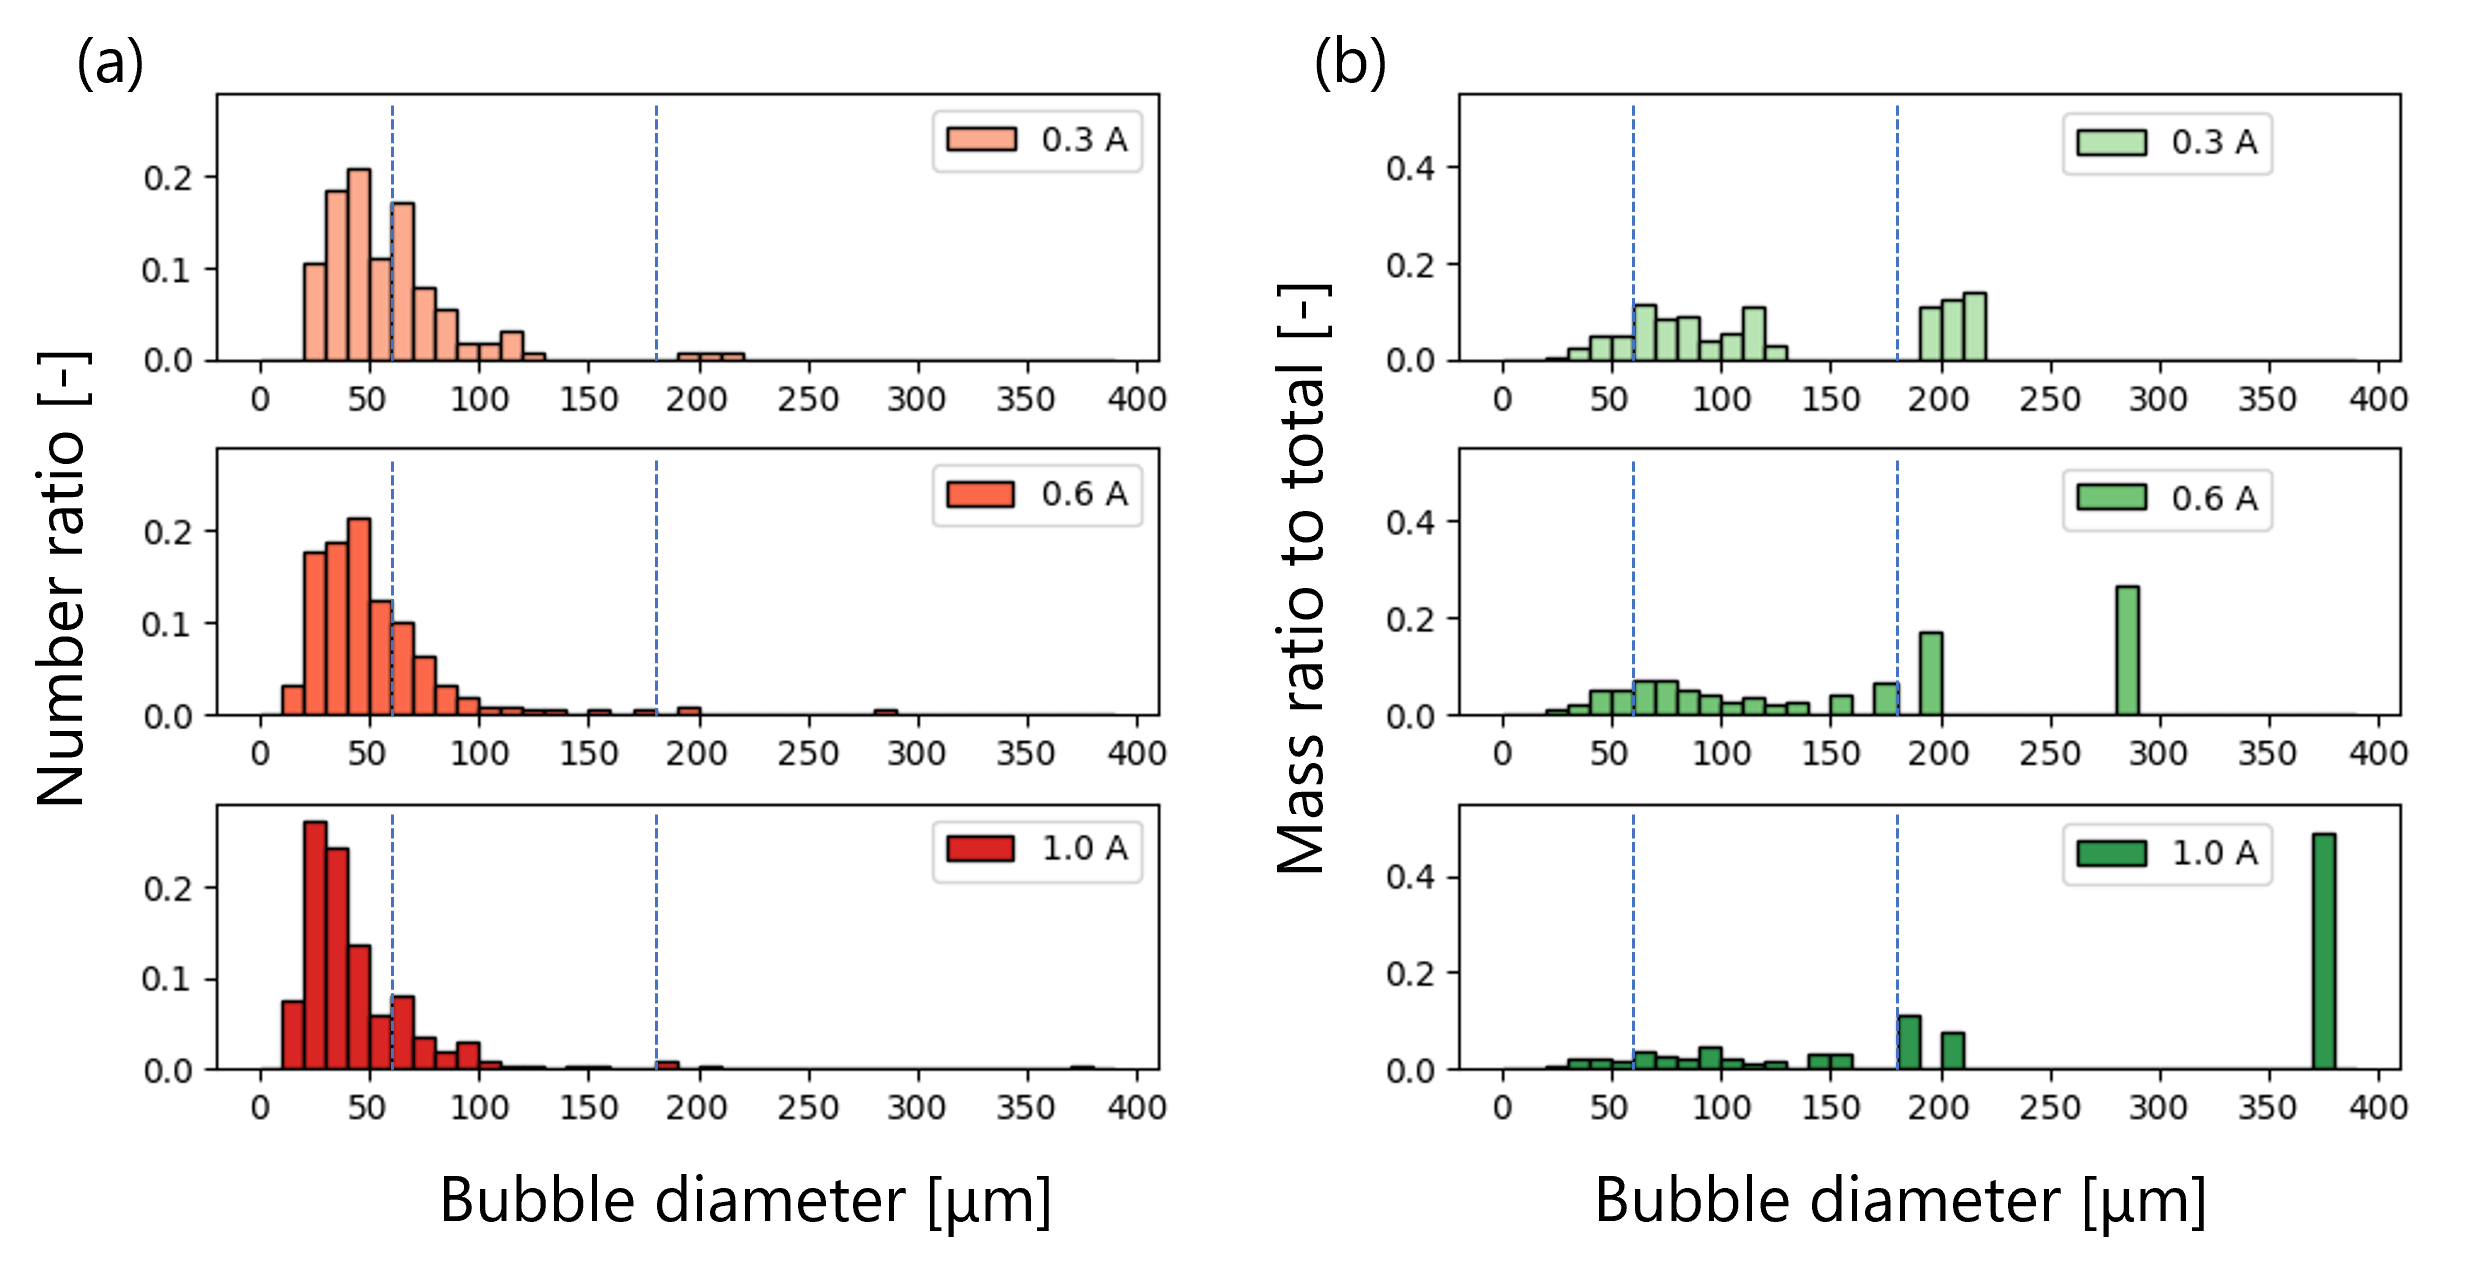
\includegraphics[width=1\linewidth]{Untitled 2.png}
  \caption{Histograms of (a) bubble diameter distribution and (b) mass ratio to the total mass. The blue dot lines show the size class boundaries: $60\,\si{\micro\metre}$ for the boundary between X1 and X2, and $180\,\si{\micro\metre}$ for the boundary between X2 and X3}
  \label{fig:histogram}
\end{figure}
\begin{figure}[h]
  \centering
  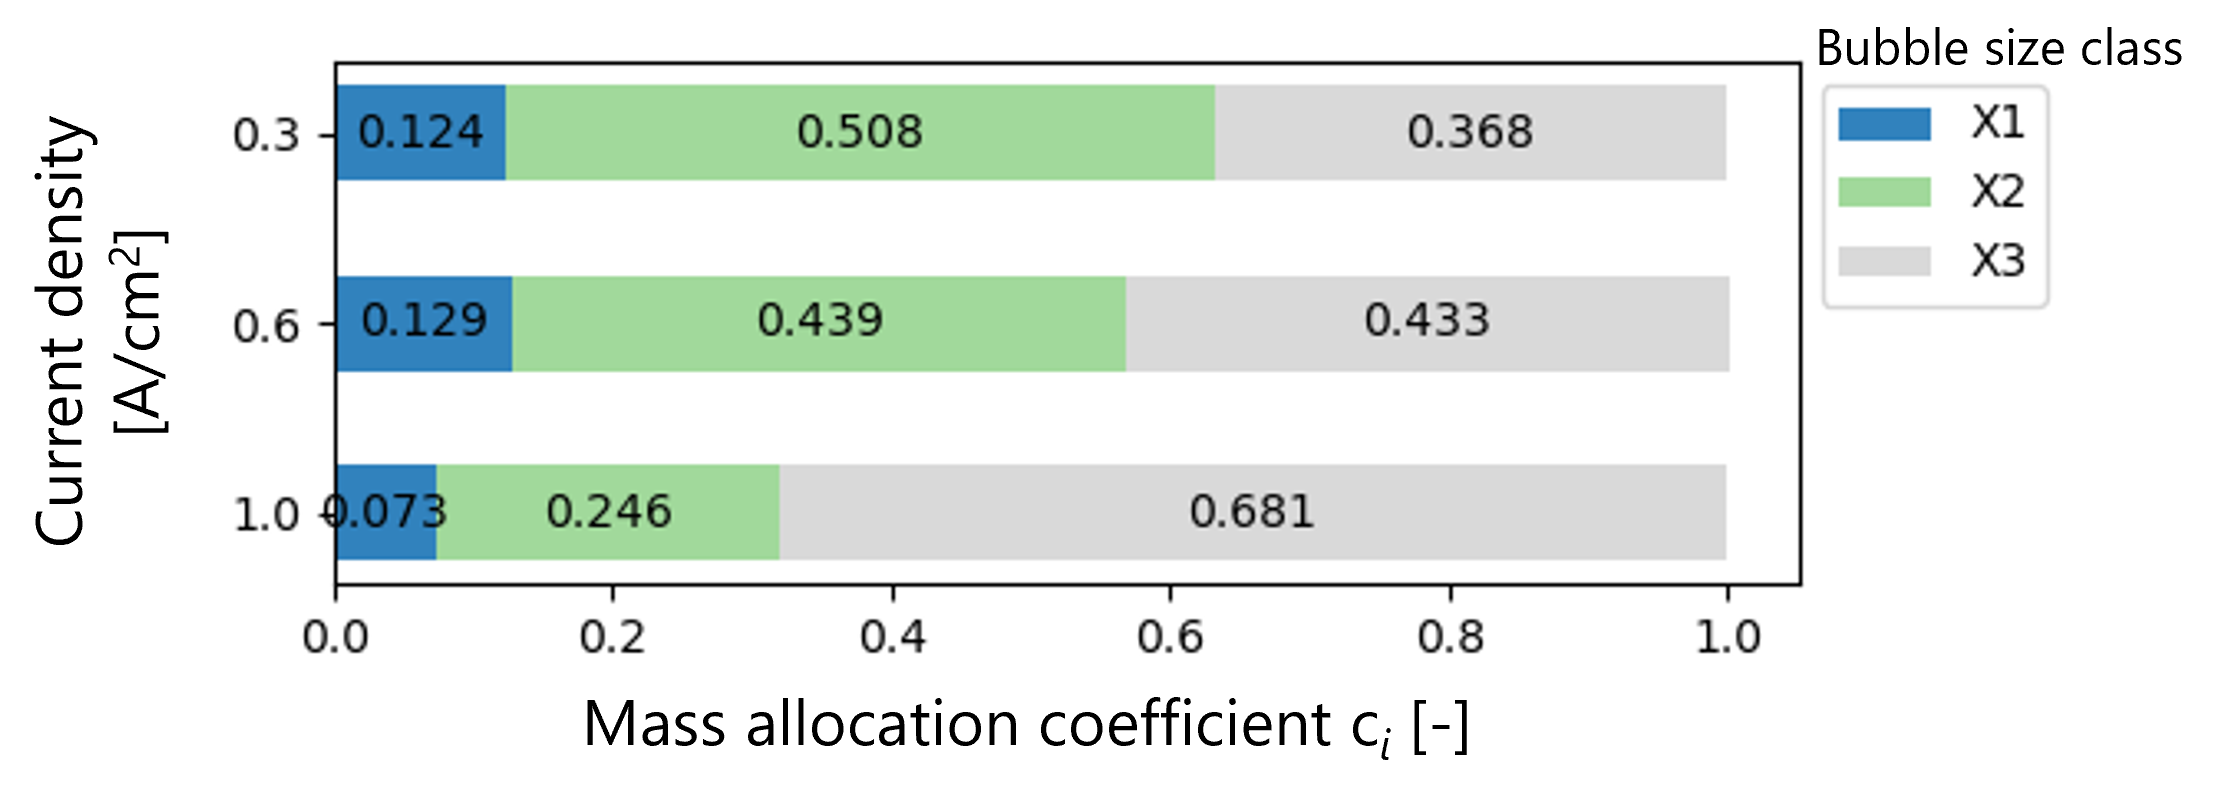
\includegraphics[width=1\linewidth]{Untitled 3.png}
  \caption{The mass allocation coefficients for size classes at each current density.}
  \label{fig:ci}
\end{figure}

\section{Results and discussion}
In Fig. \ref{fig:06Alpha}, the transition of the volume fraction field for each phase at $0.6\,\mathrm{A/cm^2}$ is illustrated.
Due to the cell's structure, the liquid phase formed a circulating flow.
Size class $\mathrm{X1}$ flowed along the liquid circulation, while $\mathrm{X3}$ flowed directly out into the outlet without circulating, and the flow field of $\mathrm{X2}$ exhibited characteristics of both $\mathrm{X1}$ and $\mathrm{X3}$.
This difference is primarily explained by the balance between drag and buoyancy, which are proportional to the square and cubic of the bubble diameter, respectively.
The specific surface area of the bubble plays a key role in the flow field. The smaller the bubble, the larger its specific surface area, making it easier to flow along the liquid phase.
This trend was similarly observed in the calculations at $0.3$ and $1.0\,\mathrm{A/cm^2}$.
\begin{figure}[h]
  \centering
  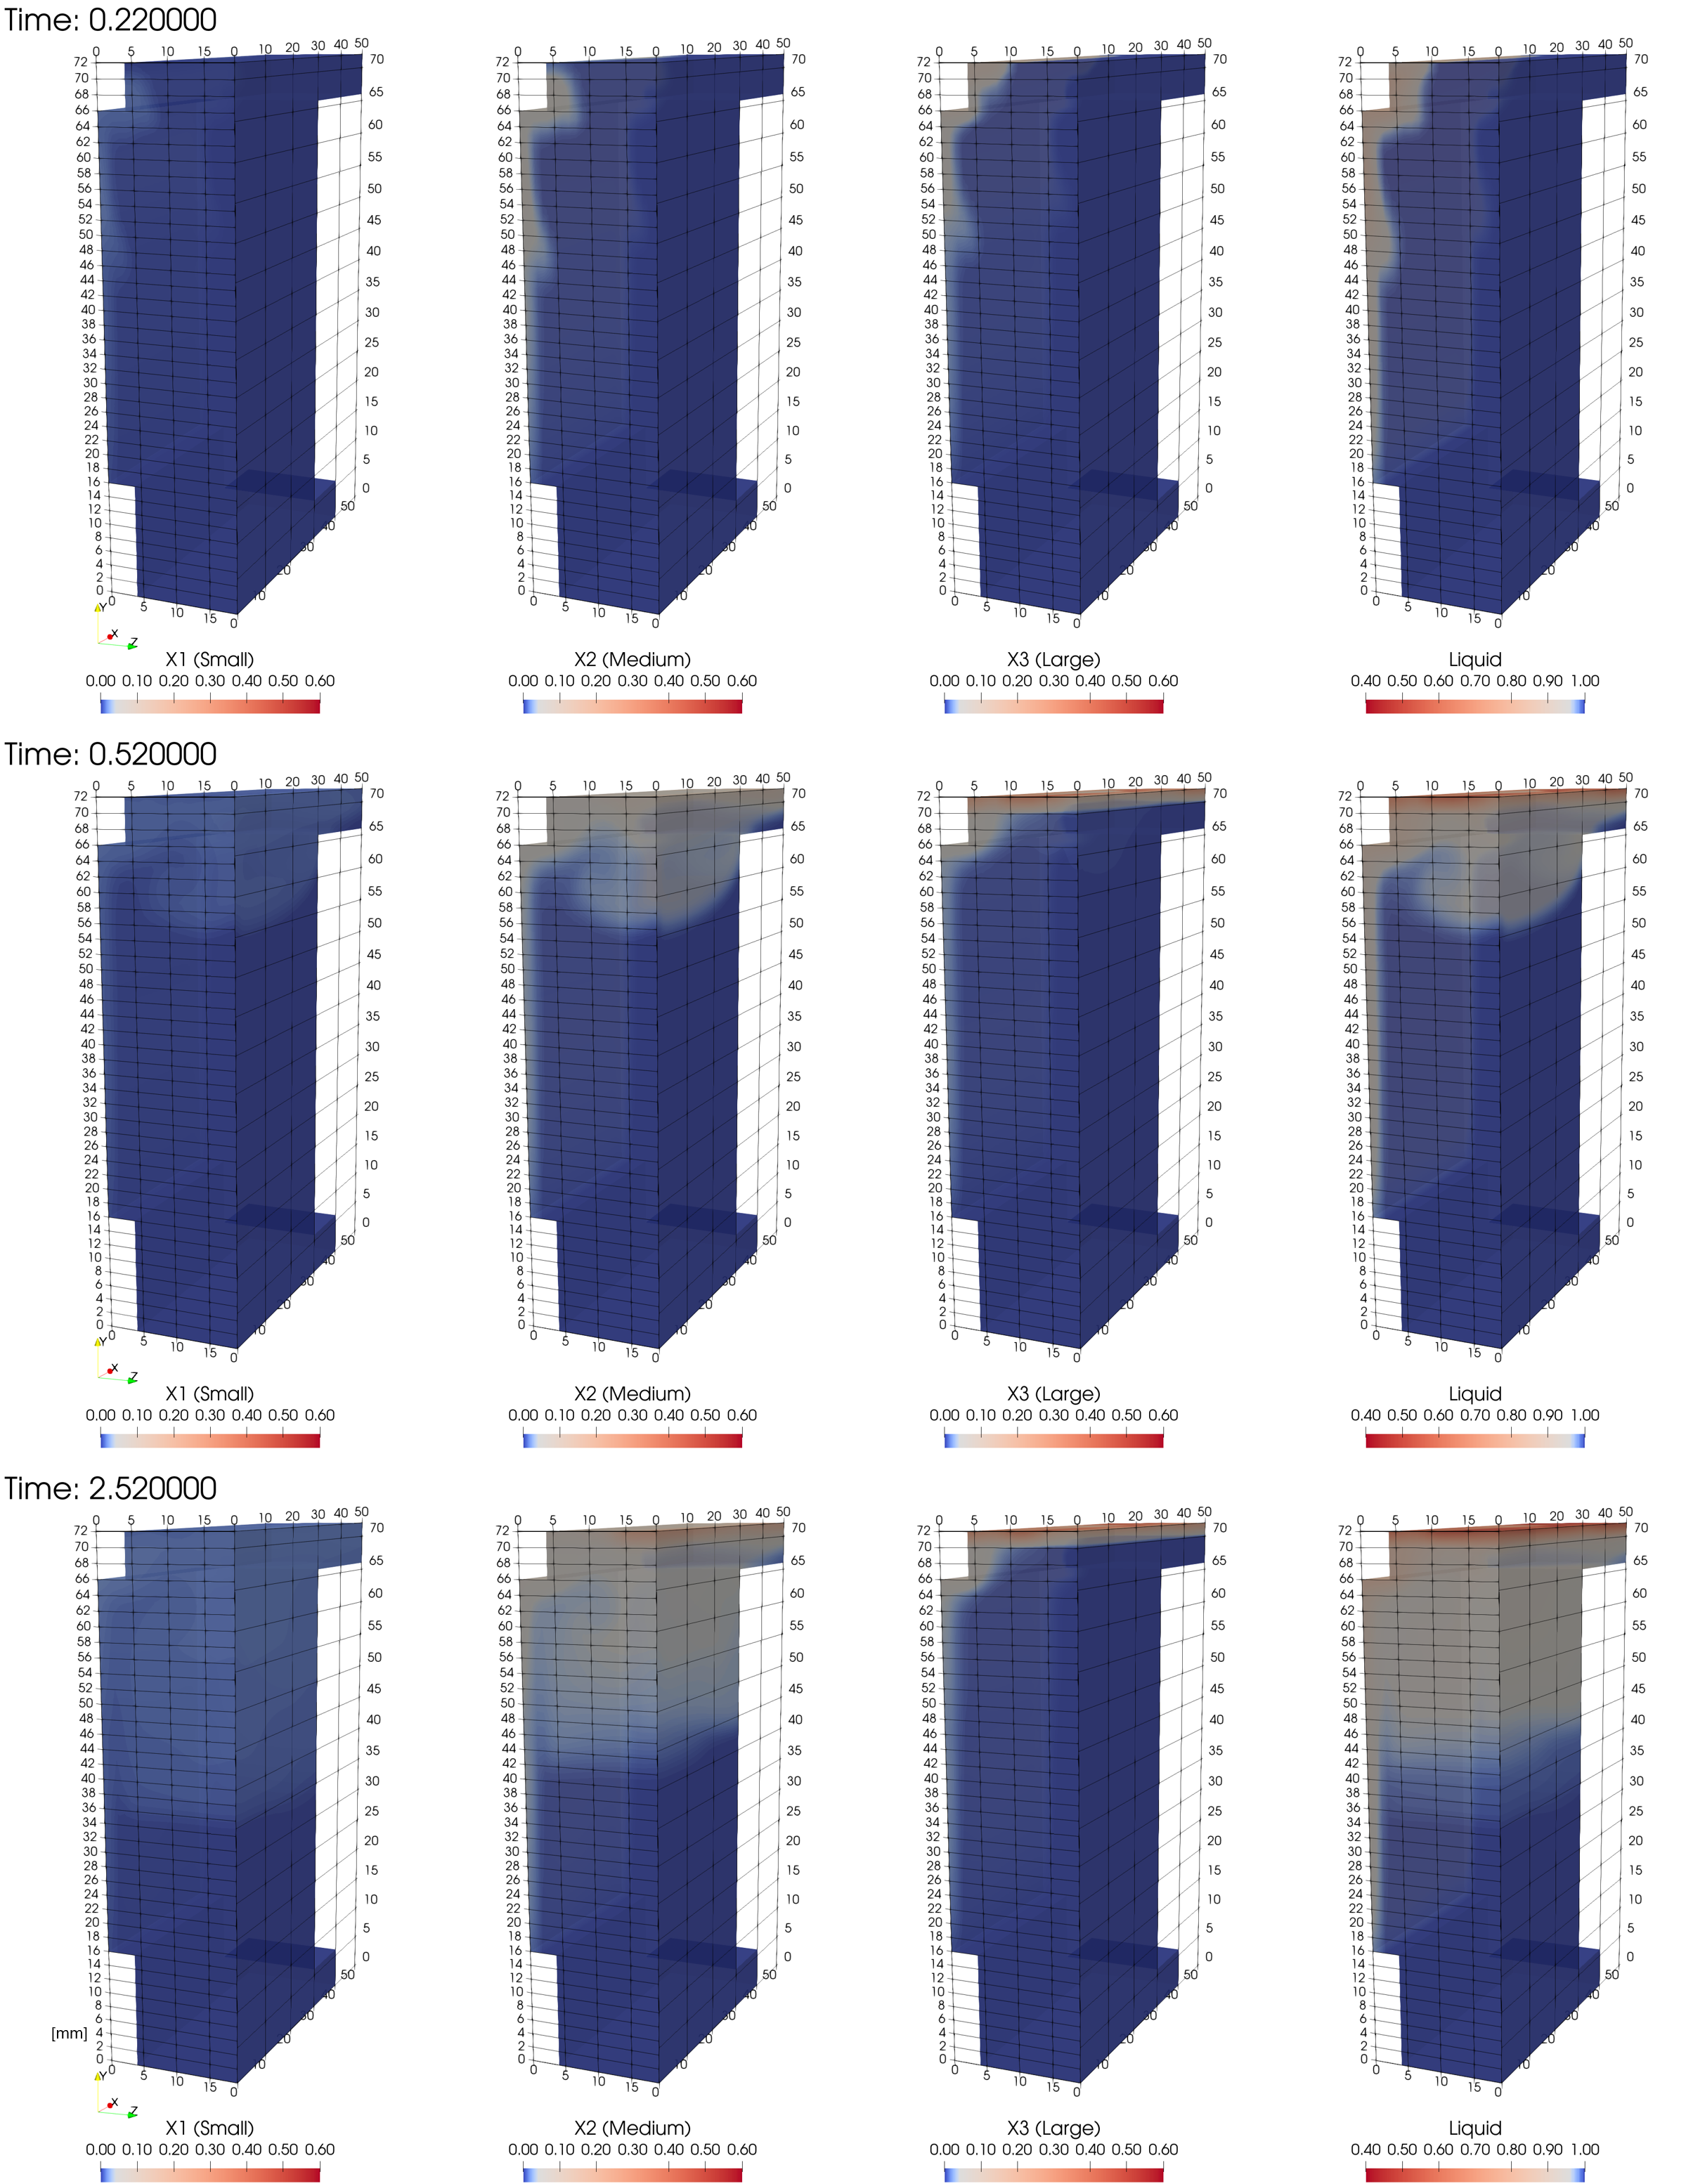
\includegraphics[width=1\linewidth]{transition_06A.png}
  \caption{The phase volume fraction fields for each bubble size class and the liquid phase at $t=0.22,\,0.52,$ and $2.52\,\mathrm{s}$.}
  \label{fig:06Alpha}
\end{figure}

The appreciable difference observed among different current densities was in the height of the bubble circulating flow, which we define as the length measured along y-direction from the top surface of the geometry to the bottom end of the bubble circulating flow.
This was compared to the experimental visualization as shown in Fig. \ref{fig:sidecomp} c.
The flow inside the cell was visualized from the side during the steady operation at each of three current densities.
In a video, the height of the bubble circulating flow fluctuated, which made the comparison complex, so the $20$ seconds of it was time-averaged to a single picture and converted into a gray-scale image.
On the other hand, as for the simulation figure, to compare it to the experimental visualization, the volume fraction field at each current density was averaged over $x$-direction from $x=0$ to $x=30\,\mathrm{[mm]}$.
In the experiment, the bubble pool volume at the top grew as the current density increased, but in the simulation, the top surface of the geometry was defined to be the same height as the top surface of the outlet hole, which is indicated by the top end of the line A-A' in Fig. \ref{fig:sidecomp}b and c.
The gas volume fractions (GVF) (Fig. \ref{fig:sidecomp}a) from the simulations, and the brightness values (BV) (Fig. \ref{fig:sidecomp}d) from the experimental images were obtained as the profiles on the line A-A'.
To compare the height of the bubble circulating flow, we focused on the position where the GVF and the BV drop to the minimum values in the range of the solid lines in Fig. \ref{fig:sidecomp}a and d.
Note that comparing the absolute values of the BVs among the different current densities is not simple because the changes in the BV do not always translate linearly into the GVF.
Therefore, the absolute values of BV among different current densities are not compared, and accordingly, the scale of each plot is adjusted so that the widths of the purple dash-dot lines in Fig. \ref{fig:sidecomp}d are consistent across the different current densities.
This scale adjustment was also applied to the plots in Fig. \ref{fig:sidecomp}d.
From Fig. \ref{fig:sidecomp}a and d, the simulation successfully reproduced the increase in the height of the bubble circulating flow.
However, as the current density increased, the simulated height of the bubble circulating flow was slightly overestimated compared to the experimental one. We consider this is because the simulation didn't take into account the bubbles trapped into the bubble pool and eventually discharged into the air from the top outlet.
This problem can be handled by incorporating bubble coalescence and breakage or assigning appropriate boundary conditions to the top surface.
\begin{figure}[h]
  \centering
  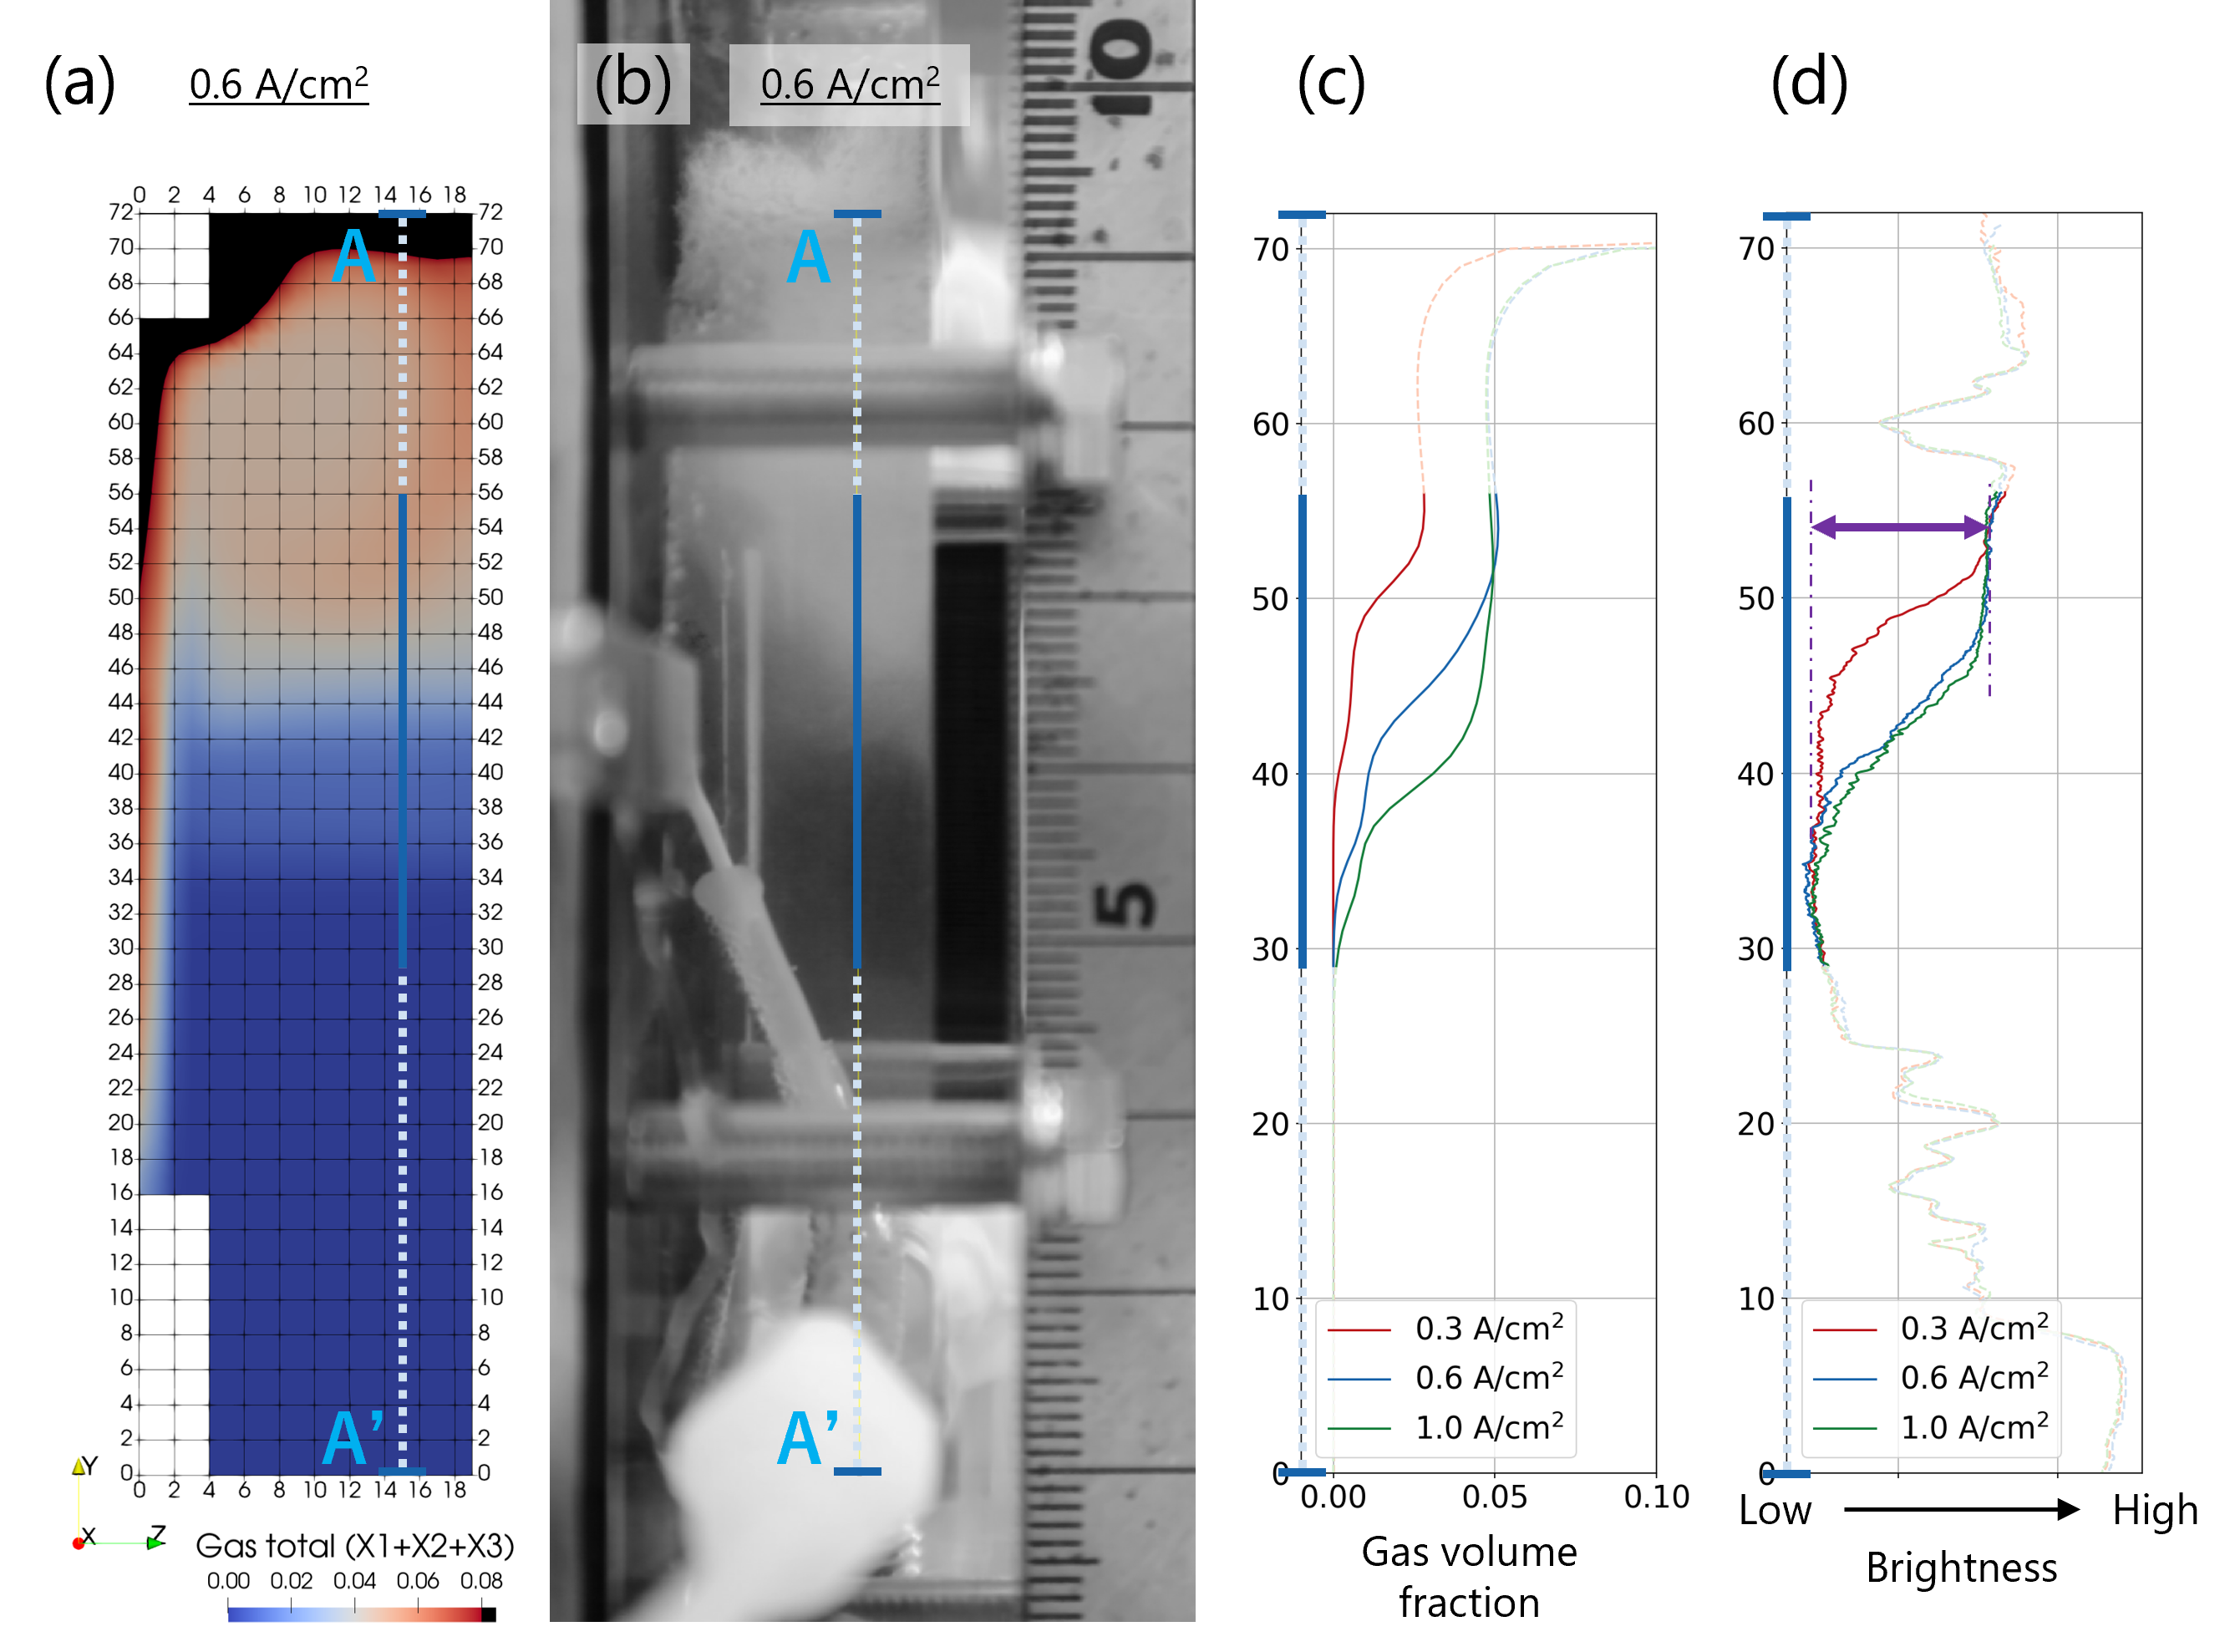
\includegraphics[width=1\linewidth]{Untitled 7.png}
  \caption{Comparison of simulation results and the experimental visualization: (a) simulated liquid volume fraction field averaged over the electrode width ($30 \mathrm{mm}$) at $0.6\ \mathrm{A/cm^2}$, with the volume fraction above 0.08 excluded from color legend, (b) experimental visualization time-averaged over 20 seconds at $0.6\ \mathrm{A/cm^2}$, (c) the gas volume fraction profiles on line A-A' of simulations at each current density, and (d) the brightness value profiles on line A-A' from the experimental visualizations at each current density.}
  \label{fig:sidecomp}
\end{figure}

As explained in Section \ref{sec:intro}, the advantage of the presented method over CFD-PBM coupled models is that it is easier to simulate flow systems where there are significant differences in velocity fields depending on the different sizes of the dispersed phase.
Here, to demonstrate the advantage of the presented method, a simulation with only medium size bubble (named simulation ``M'') was performed and the liquid volume fraction on the surface of the electrode was compared to that of the simulation with three bubble sizes (named simulation ``SML'').
Fig. \ref{fig:alphaElectrode} shows the plots of average liquid volume fraction (ALVF) over time in the lower ($y=20$ to $30\,\mathrm{[mm]}$, $z=0$) and upper ($y=50$ to $60\,\mathrm{[mm]}$, $z=0$) area selections on the electrode surface.
\begin{figure}[h]
  \centering
  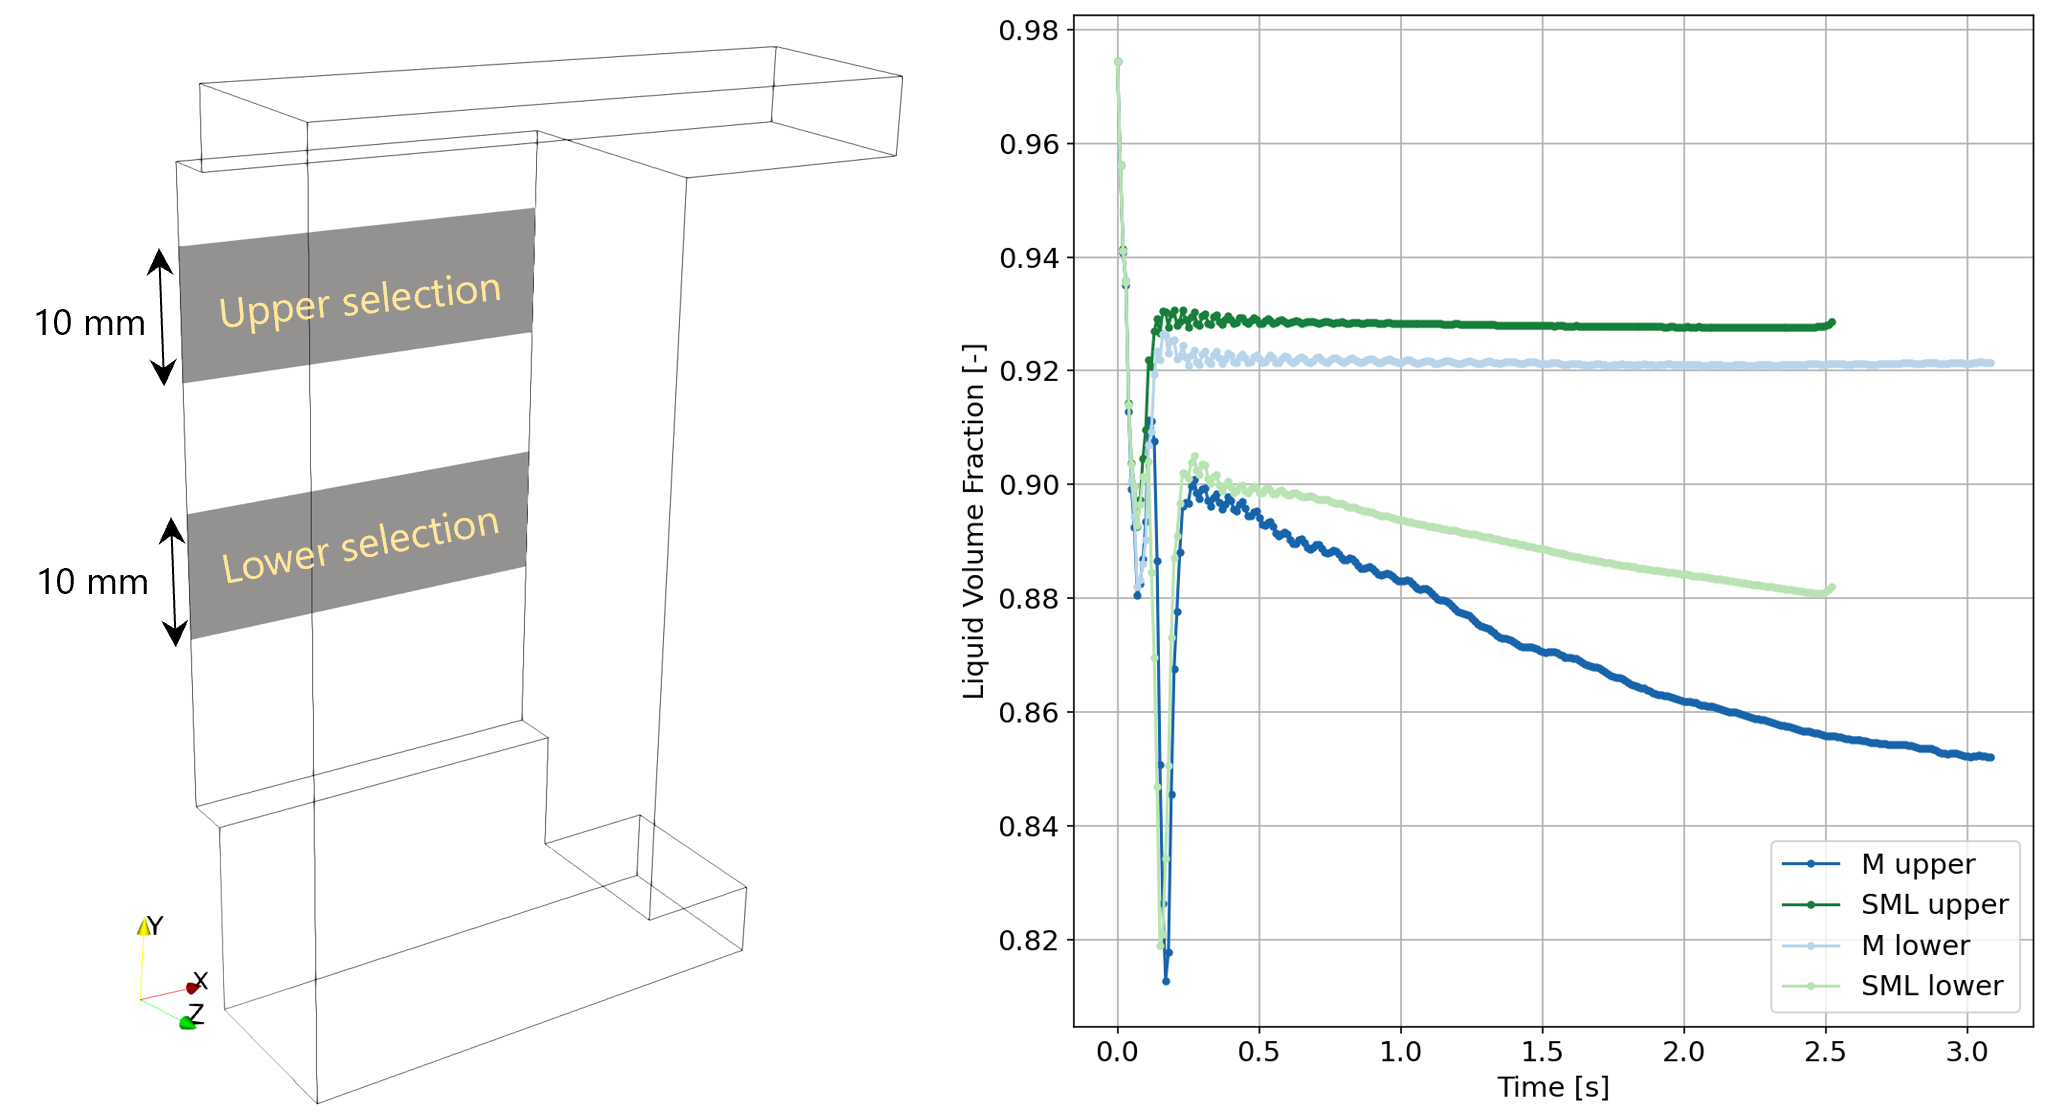
\includegraphics[width=1\linewidth]{Picture2.png}
  \caption{Comparison of the average liquid volume fraction on the two selected areas over time between the simulation with three bubble size classes (``SML'') and that with one bubble size class (``M'') at $1.0\ \mathrm{A/cm^2}$}
  \label{fig:alphaElectrode}
\end{figure}
The ALVFs drop right after bubble generation ($t=0$ to $t\approx0.1\,\mathrm{[s]}$) for both the upper and lower selections in the two simulations.
Subsequently, in the upper selection, the ALVFs further decrease owing to rising bubbles from the lower part of the electrode.
Eventually, for both the upper and lower selections, the ALVFs begin to increase and settle to almost constant values.
Overall, simulation ``M'' underestimates the ALVF compared to simulation ``SML''.
This comparison suggests the importance of considering multiple sizes for the dispersed phase.

\section{Summary}
Achieving more precise predictions of bubble flow is crucial for the design of high-performance water electrolyzers.
The treatment of dispersed bubble size significantly influences the simulation results.
While monodisperse models commonly used for predicting bubble flow in water electrolysis cells often yield inadequate predictions, there is a lack of examples utilizing the polydisperse model, such as the Population Balance Model (PBM), for simulating bubble flow including circulating flow inside water electrolysis cells.

In this study, a new model was proposed that classifies the dispersed gas bubble phase into mulitiple bubble size classes based on bubble diameter and calculate individual velocity and volume fraction fields for each size class.
This model successfully simulated distinct flow fields of each size class, which is attributed to differences in their specific surface areas.
The simulation results were validated against experimental visualization for several current densities.
Furthermore, using this model, a simulation with multiple size classes and that with a single size class were compared, confirming differences in their bubble volume fractions in the vicinity of the electrode surface.

\section{Acknowledgements}
This study was based on results obtained from the Development of Fundamental Technology for Advancement of Water Electrolysis Hydrogen Production in Advancement of Hydrogen Technologies and Utilization Project (JPNP20003) commissioned by the New Energy and Industrial Technology Development Organization (NEDO).

%% The Appendices part is started with the command \appendix;
%% appendix sections are then done as normal sections
%% \appendix

%% \section{}
%% \label{}

%% If you have bibdatabase file and want bibtex to generate the
%% bibitems, please use
%%
%%  \bibliographystyle{elsarticle-num} 
%%  \bibliography{<your bibdatabase>}

%% else use the following coding to input the bibitems directly in the
%% TeX file.

\bibliographystyle{elsarticle-num}
\bibliography{AWEsim}

%\begin{thebibliography}{00}
%
%%% \bibitem{label}
%%% Text of bibliographic item
%
%\bibitem{}
%
%\end{thebibliography}
\end{document}
\endinput
%%
%% End of file `elsarticle-template-num.tex'.
